

\chapter{Bureaucratic Intermediation \& Urban Water Governance: Evidence from Lucknow and Bhopal \\ \large December 16, 2024}\footnote{This is the fourth chapter of the dissertation and the third empirical chapter. Chapter 2 analyzes citizen survey data to assess access to water and trash services and interactions with the bureaucratic and political systems mediating service delivery. Chapter 3 examines trash as a public good, using ethnographic research and comparative historical analysis to explore mechanisms of public goods delivery across two cities. Chapter 1 and Chapter 5 are introductions and conclusions.}

\clearpage % Forces all subsequent content to the next page

\date{}

\pagebreak
Note for Comparative and Multi-Method Approaches within Political Economy Research


The “water chapter” is a pivotal empirical chapter in my dissertation on “Bureaucracy, Politics, and Development.” It fits into the broader project as one of two in-depth comparative case studies (the other focuses on trash management ), and it specifically examines how bureaucratic and political dynamics affect the delivery of urban water services in Bhopal and Lucknow. Together with a quantitative survey chapter, these case studies form a triad of evidence supporting the dissertation’s overarching argument about local state capacity. The water chapter provides a sector-specific lens to test and illustrate the dissertation’s theoretical claims. In essence, it asks: Why did Bhopal achieve broader access to piped water than Lucknow under similar conditions, and what does this tell us about governance?
By zooming in on water provision – a classic public good that is essential, highly visible, and politically salient – this chapter sheds light on the mechanisms behind uneven development outcomes. Water supply is not only a technical challenge but also a political one: it requires coordination across agencies, steady infrastructure investment, and fair distribution, making it an ideal domain to study state capacity and performance legitimacy at the city level. The water chapter’s findings complement those from the trash case, reinforcing the dissertation’s comparative insights while highlighting unique aspects of the water sector.

A Rich Mixed-Methods Approach in One Case Study
The water chapter exemplifies the mixed-methods approach of the dissertation, leveraging multiple sources of evidence to build a compelling case. It draws on qualitative, quantitative, and historical data at multiple levels of analysis. Key methodological components include:
Ward-Level Comparisons and Local Case Histories: 

Within each city, the chapter delves into specific urban wards and neighborhoods to compare water service outcomes and local governance dynamics. For instance, it contrasts a well-served ward in Bhopal with a poorly served counterpart in Lucknow, illustrating how local leadership and civic engagement interacted with institutional constraints. These fine-grained ward studies make the analysis concrete and grounded, capturing variation within cities that aggregate statistics might obscure.


Ethnographic Interviews Across Bureaucratic Hierarchies: I conducted dozens of interviews with stakeholders in the water sector – from senior bureaucrats in state water agencies and municipal commissioners, to mid-level engineers and frontline staff like ward-level officials and plumbers, as well as elected city councilors. This ethnographic fieldwork uncovered how actors at different levels perceive the problems and navigate them. Crucially, it revealed the presence of intermediary bureaucrats in Bhopal who coordinated between state and city authorities, versus their absence in Lucknow. One mid-level engineer in Lucknow described the city’s water governance as “Trishanku-like,” meaning suspended in an uncertain state between multiple masters, highlighting the institutional fragmentation that my research documents. These on-the-ground perspectives give life to the formal organizational charts, showing how rules and roles translate (or fail to translate) into action.


Household Survey Data on Service Access: The chapter incorporates quantitative evidence from an original household survey (jointly analyzed in Chapter 2 of the dissertation) to demonstrate the outcome differences in water provision. The survey covered representative samples of households across various wards in both cities. It found striking disparities: by 2022, 87% of households in Bhopal had access to piped water, compared to only 72% in Lucknow . Additionally, residents in Lucknow reported shorter supply hours and heavier reliance on private wells or tankers. Such data substantiates the claim that Bhopal achieved a higher level of service coverage – the puzzle that qualitative analysis seeks to explain. The survey evidence strengthens the chapter’s argument by showing that the differences are not anecdotal but systematic. It also allows me to rule out certain alternative explanations (for example, differences in population wealth or demand) by controlling for them in the analysis .


Comparative-Historical Process Tracing: To understand how these divergences came about, the water chapter traces each city’s institutional and policy evolution over the last ~30 years. I identify critical junctures when major water sector reforms or investments were attempted, such as the late 1990s state-level decentralization reforms and the mid-2000s national urban renewal mission. The chapter compares how Bhopal and Lucknow responded at these junctures. In Bhopal, for example, a World Bank-funded water project in the early 2000s was leveraged by reform-minded bureaucrats to establish new procurement norms and embed a project management unit directly within the municipal structure. This created a precedent for greater city-level capacity. In contrast, Lucknow’s attempt to implement similar reforms faltered: the water utility (the Lucknow Jal Sansthan) remained caught between the state government’s Jal Nigam and the municipal corporation, never gaining the autonomy or cohesion needed to implement improvements. Archival documents and interviews with retired officials detail how repeated reform efforts in Lucknow were derailed by turf wars between agencies and lack of political follow-through, whereas Bhopal benefited from a somewhat more unified administrative mandate. By chronicling these paths side by side, the chapter shows that today’s outcomes are products of path-dependent processes, not just one-off events.


Overall, the water chapter presents a layered analysis: it moves from macro-level comparisons (citywide service coverage rates and institutional forms) to the meso-level (agency interactions and policies over time) down to the micro-level (ward conditions and individual actors’ experiences). This triangulated approach within a single chapter exemplifies the value of mixed methods. Each type of evidence reinforces the others – for instance, statistical differences prompt deeper inquiry into institutional causes, while ethnographic findings about bureaucratic behavior give plausible explanations for the numbers. By integrating these pieces, the chapter provides a 360-degree view of the political economy of water provision in the two cities.
Insights into Public Service Delivery and State Capacity
The substantive findings of the water chapter underscore themes that lie at the heart of political economy debates on development – making it a perfect fit for a workshop on mixed-methods approaches to these issues. A central insight is that institutional context and bureaucratic agency mediate service delivery outcomes in crucial ways. Bhopal and Lucknow had comparable formal structures on paper (both draw from the same state-cadre bureaucracy and legal framework ), yet their performance diverged because of differences in how politicians and bureaucrats interacted in practice. In Bhopal, a cohort of bureaucrats exercised what I term “conditional autonomy”: they had enough independence to enforce technical standards and pursue inclusive policies, while still bending where necessary to accommodate political pressures . This delicate balance – neither full insulation nor outright politicization – allowed them to push toward what I call “precarious universalism,” meaning near-universal service coverage achieved through incremental, negotiated reforms . In Lucknow, by contrast, bureaucrats were never granted the space to innovate or assert professional authority; the water agency was neither fully under local control nor fully autonomous . This resulted in chronic paralysis: frequent turf conflicts between state and city officials, half-implemented projects, and an ad-hoc patchwork of stopgap solutions (like private tankers and handpumps) for marginalized communities  . The contrast illustrates that it is the quality of coordination between political and bureaucratic actors – whether they achieve a programmatic coalition or fall into a patronage-driven equilibrium – that largely determines service outcomes  .
These findings speak to broader political economy topics such as redistribution, public goods, and state capacity. Water is a quintessential public good, and ensuring broad access to it is a form of redistribution and social equity. The chapter shows that effective redistribution (in the form of extending services to poorer neighborhoods) depended on building local state capacity and coherence. Where bureaucratic coordination was present (Bhopal), the local state could deliver more inclusive outcomes; where it was absent (Lucknow), service delivery tended to favor those with connections or wealth, exacerbating inequality. In this way, the research connects to Patrick Heller’s argument that inequality in cities is often “produced” by state structures, not just a residual occurrence (State-produced inequality in an Indian city - CPR). As Heller and Mukhopadhyay (2015) found in Delhi, uneven access to services like water is a result of how institutions are organized and whose interests they serve (State-produced inequality in an Indian city - CPR). My water chapter provides a comparative demonstration of this principle: the institutional set-up and informal governance arrangements in each city actively shaped who gets water and who doesn’t. It thereby grounds abstract ideas of state capacity and social contracts in concrete urban governance practices.
Crucially, the chapter’s focus on performance in service delivery has implications for democratic governance. Recent scholarship has underscored that democracies gain legitimacy by delivering results for citizens (Delivering for Democracy: Why Results Matter | Journal of Democracy). In their 2025 Journal of Democracy piece “Delivering for Democracy,” Fukuyama and colleagues argue that tangible improvements in services and infrastructure are critical to restoring citizens’ faith in democratic systems amid global backsliding (Delivering for Democracy: Why Results Matter | Journal of Democracy). The story of Bhopal and Lucknow’s water systems illustrates this point at the city level. Bhopal’s relative success in expanding access can bolster citizens’ satisfaction and trust in local government, whereas Lucknow’s failures risk eroding confidence in democratic governance, as residents see the state unable to meet basic needs. This link between state performance and democratic legitimacy provides an important normative backdrop for my research. It suggests that studying how to improve service delivery is not only about efficiency or development – it is also about sustaining the credibility of democratic institutions through performance legitimacy. The water chapter, by pinpointing the governance factors that enable better performance, contributes to this wider conversation on “delivering for democracy.”
Conclusion: Advancing a Triangulated Political Economy of Development
In sum, the water chapter showcases how a rich, triangulated methodological approach can illuminate core issues in political economy. By combining deep qualitative inquiry with supporting quantitative data and historical analysis, it provides a nuanced explanation for variation in a vital public service. This approach aligns perfectly with the workshop’s theme of mixed methods: it demonstrates in practice how blending methods leads to more robust insights on topics like public service provision and state capacity. The chapter’s evidence of ward-level outcomes, human stories of bureaucrats and citizens, and decades-long institutional trajectories all reinforce one another, painting a comprehensive picture that single-method studies could easily miss.
By explicitly connecting these micro- and meso-level findings to broader themes of redistribution and governance, the chapter also illustrates the value of specificity for general debates. It takes abstract concepts – for example, the idea of a “flailing state” or a patronage equilibrium – and shows exactly how they play out in water taps running (or running dry) in real neighborhoods. This kind of specific, grounded evidence is precisely what a mixed-methods political economy approach can contribute: it validates theories against reality and uncovers mechanisms that can inform policy and further research.
Ultimately, the water chapter’s integration into the dissertation strengthens the whole project’s contributions. It ensures that the dissertation is not just theoretically informed but empirically rich and credible, drawing on multiple lenses to cross-check and enrich conclusions. For a workshop dedicated to mixed methods, this chapter will serve as an example of how and why marrying methods can be so fruitful in political economy research. It highlights that to understand complex phenomena like state capacity or service delivery, we must be willing to “get our feet wet” in multiple pools of evidence – qualitative, quantitative, historical – and weave them together. Such an approach, I argue, is key to delivering findings that are both scientifically rigorous and deeply relevant to the pressing challenges of governance and development.
Sources: Recent scholarly insights on service delivery and democracy (Delivering for Democracy: Why Results Matter | Journal of Democracy); urban governance and inequality in India (State-produced inequality in an Indian city - CPR) (State-produced inequality in an Indian city - CPR); and dissertation fieldwork and data from Bhopal and Lucknow  .


\section{Introduction: The Challenge of Urban Water Provision}

Why do some cities, operating under broadly similar policy environments and administrative frameworks, achieve more reliable public services than others? Consider the divergent experiences of two Indian cities, Bhopal and Lucknow. Both function within comparable legal mandates, rely on bureaucrats drawn through state-level competitive exams, and have access to national and international funding streams for water infrastructure. From 1981 through 2001, their trajectories in household tap water access ran parallel. Yet by 2022, while Bhopal provided piped water to 87\% of its households, Lucknow reached only 72\% (Figure 1.1) . Conventional factors—resource allocations, partisan alignments, or formal organizational structures—offer incomplete explanations for this gap.

\begin{figure}[H] % Use [H] to force the image to appear exactly where you place it
    \centering
    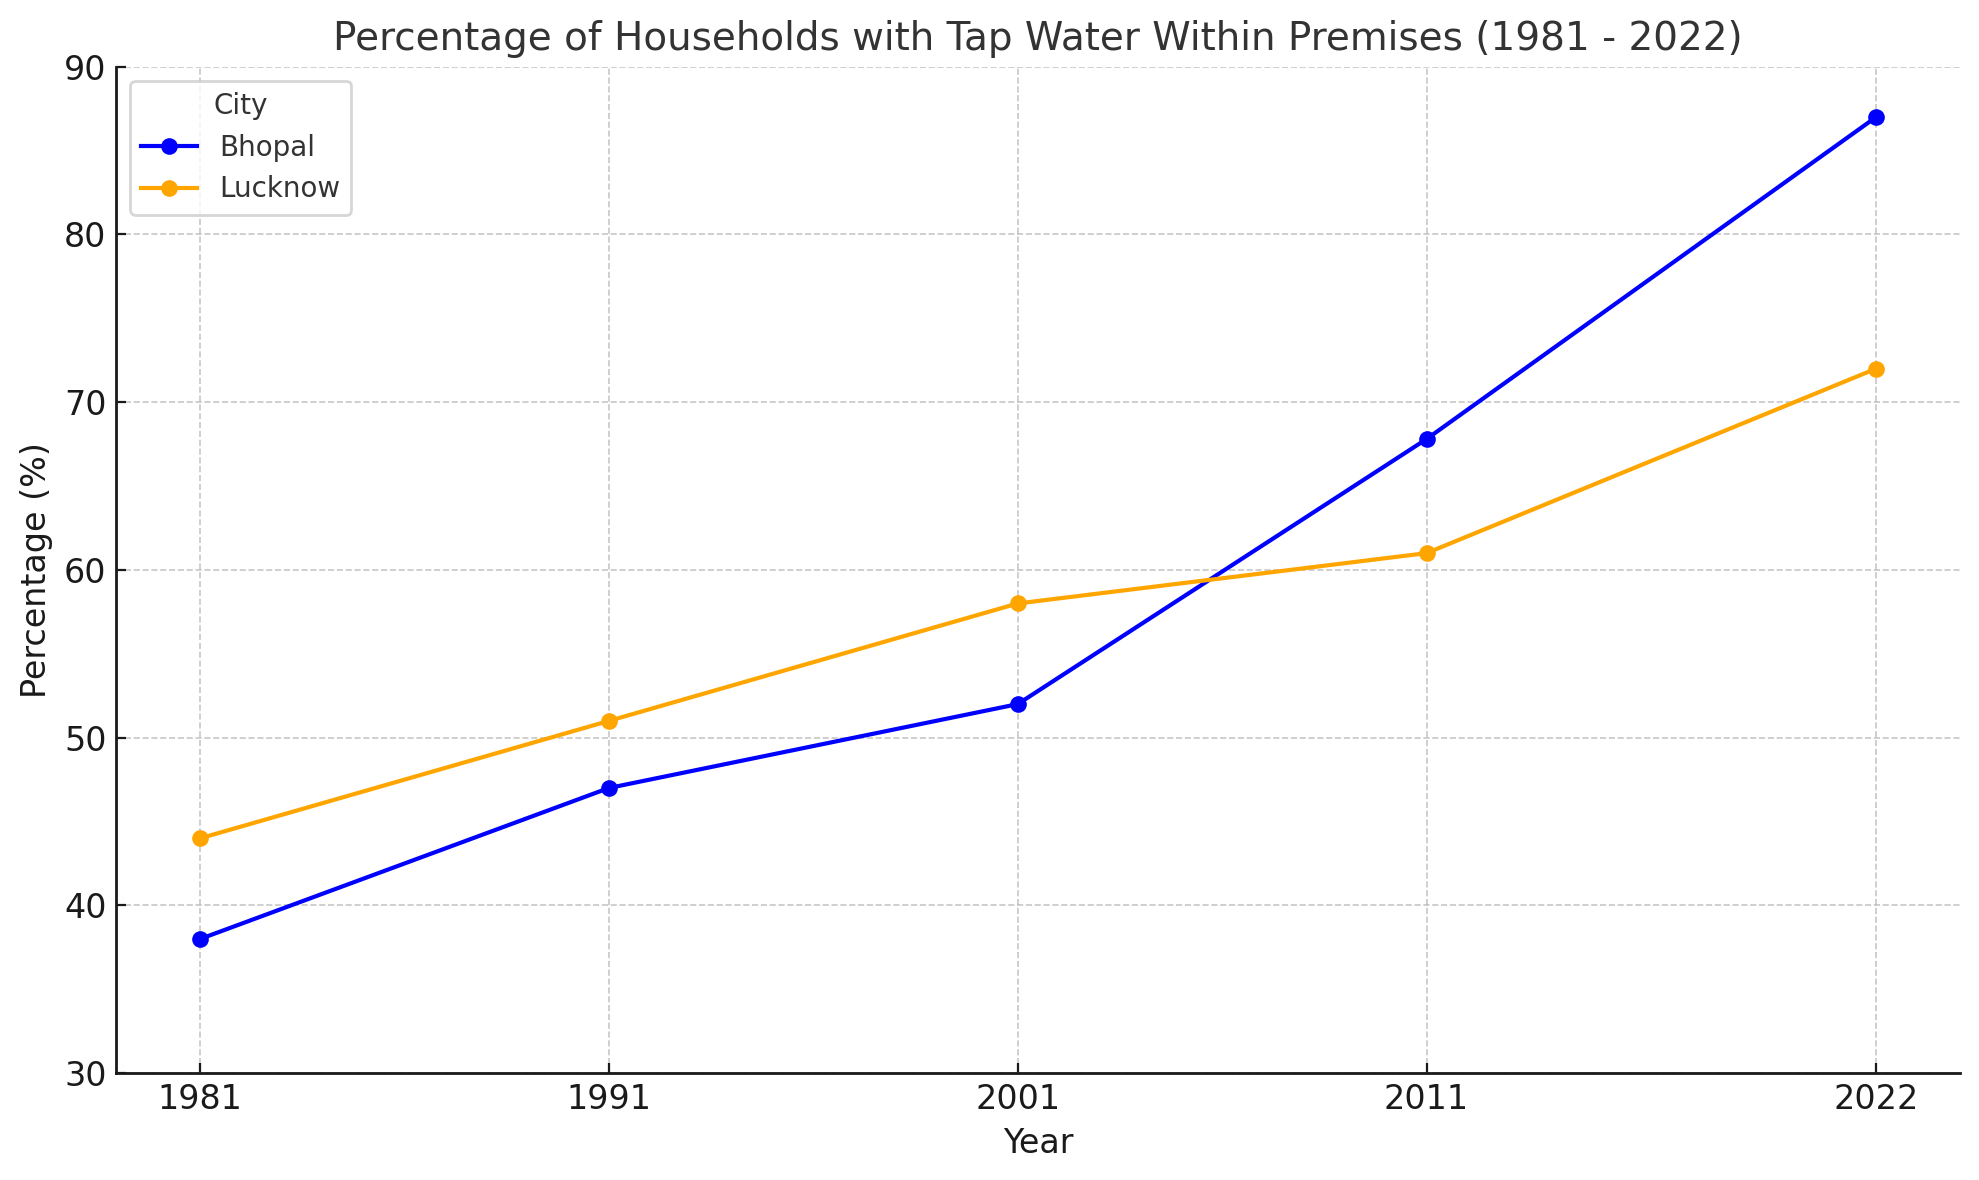
\includegraphics[width=.8\textwidth]{images/diff.png} % Adjust the width as needed
    \caption{Change in Tap water across Bhopal and Lucknow. Data for 1981-2011 is from the
Census of India, 2022 is from Primary Household Survey.}
   
\end{figure}

This chapter argues that the key determinant lies not in the formal characteristics of bureaucratic recruitment or tenure, but in how state-level bureaucrats mediate between political pressures and technical imperatives. These officials, positioned between elite policymakers and frontline implementers, play a crucial role in translating policy into practice. In Bhopal, state-level bureaucrats operated under what I term ``conditional autonomy" – sufficient operational independence to maintain technical standards while accommodating legitimate political demands. This enabled them to manage political-business relationships effectively, and legitimize community-driven solutions. The result was what I call "precarious universalism": broad service coverage that, while imperfect, proved more sustainable than alternative arrangements.

In contrast, Lucknow's water utility body, the Lucknow Jal Sansthan (LJS), remained trapped in what local officials describe as a ``\textit{Trishanku}-like" state – neither fully integrated into municipal governance nor granted meaningful autonomy. Despite having bureaucrats with similar professional backgrounds and protections as their Bhopal counterparts, LJS officials could not forge conditions for receiving  conditional autonomy necessary for effective service delivery. This resulted in persistent institutional paralysis, characterized by unresolved authority conflicts between state and city body, failed reform attempts, and reliance on informal, often inequitable solutions.

The comparative analysis reveals that successful service delivery depends not just on formal institutional designs, bureaucratic recruitment patterns, or resource allocation, but on bureaucrats' capacity to navigate complex political-administrative terrain. Where state-level officials can build coalitions, moderate competing interests, and institutionalize problem-solving routines, they create conditions conducive to improved service delivery – even without achieving ideal-type programmatic governance.

This argument advances our theoretical understanding of state capacity in three ways. First, it introduces the concept of \textit{conditional autonomy}, showing how bureaucrats can advance service delivery, even absent idealized Weberian conditions. Second, it highlights the distinct role of state-level bureaucrats as \textit{intermediaries within the state} apparatus, shifting focus from external brokers emphasized in previous research. Finally, it demonstrates how different forms of political-bureaucratic relationships produce varying service delivery outcomes, ranging from \textit{fragmentation to precarious universalism}.

The evidence presented comes from extensive fieldwork, including interviews with bureaucrats, politicians, and community leaders; analysis of administrative records; and a representative household survey comparing service access across both cities. This empirical foundation reveals how bureaucratic intermediation shapes not just project implementation but the broader patterns of urban service delivery, offering insights for understanding state capacity in developing contexts.


\section{Theory: Conditional Autonomy and Service Delivery}

Much of the literature on urban service provision frames governance in dichotomous terms: either programmatic policies delivered through impartial, rule-bound bureaucracies, or patronage-driven arrangements that reward political supporters \citep{pepinsky_bureaucracy_2017, kitschelt_patrons_2007-1}. In an idealized scenario, programmatic politics and autonomous bureaucracies would ensure predictable, universal access to public goods. Yet, across the Global South, such ideal types rarely materialize. Instead, cities more commonly exhibit hybrid conditions—arrangements that resist neat classification and combine elements of both programmatic and patronage-based governance.

Existing research acknowledges this hybridity. A robust body of work has explored the role of non-state intermediaries—brokers, party workers, and local leaders—who help citizens secure discrete, easily targeted goods like streetlights, ration cards, or communal water standposts\citep{auerbach_demanding_2019, krishna_politics_2007, pande_can_2011}. While these actors can alleviate immediate needs, their interventions often remain limited to small-scale, non-networked services. They rarely spur the coordinated, citywide improvements required by infrastructure-intensive public goods such as piped water or sewage systems. Moreover, dependence on these outside-the-state intermediaries can entrench fragmented patterns of provision, discouraging the state from assuming direct responsibility for long-term solutions. Thus, while brokers can deliver incremental benefits, they typically fail to foster comprehensive or equitable systems of public service delivery. Therefore, to understand how cities can achieve more stable and equitable outcomes, we must re-center the analysis on actors within the state -- specifically relationships between politicians and bureaucrats operating within formal government structures.


\subsubsection{Defining Conditional Autonomy}

By conditional autonomy, I refer to a configuration in which bureaucrats, embedded in political contexts rich in patronage and informal practices, secure a measure of professional discretion and normative standing, yet fall short of achieving the full institutional insulation or legal-rational coherence characterizing classic Weberian bureaucracies \citep{weber_max_1946, evans_government_1996}. In contrast to idealized portrayals of bureaucrats as uniformly rule-bound and shielded from political interference, conditional autonomy emerges amid ongoing negotiation and selective compromise between bureaucrats and political elites \citep{migdal_strong_1988, heller_labor_1991}. Key Features of Conditional Autonomy:

Partial Insulation:
Rather than being categorically free from political interference, bureaucrats maintain a circumscribed space for technical judgment. This partial insulation may derive from professional reputation, informal understandings, or the ability to leverage limited but salient points of resistance to politically motivated directives \citep{grindle_divergent_1997, tsai_accountability_2012}. Although not absolute, these forms of insulation temper capricious interventions and uphold minimal technical standards.

Strategic Adaptation:
Bureaucrats exercise agency through selective accommodation and resistance, strategically yielding on issues like incremental resource deployment or minor policy adjustments to safeguard core domains of technical integrity and long-term planning \citep{pepinsky_bureaucracy_2017, auerbach_clients_2019}. In doing so, they skillfully navigate a terrain of shifting alliances and informal deals, maintaining enough leeway to incrementally improve service delivery outcomes despite persistent patronage pressures.

Incremental Norm-Building:
Over time, the pragmatic engagements that constitute conditional autonomy help consolidate informal norms of professional conduct and create a shared understanding of acceptable interventions. Repeated bargaining episodes not only stabilize expectations but also generate incremental improvements in administrative routines, contributing to more predictable patterns of political-bureaucratic exchange \citep{levi_rule_1988, fukuyama_governance:_2016}.

Capacity Enhancement Under Constraint:
Conditional autonomy’s viability improves through modest but meaningful investments in administrative capacity, such as better data systems, procurement reforms, and targeted training. These measures enhance the bureaucracy’s credibility and negotiating power, enabling it to insist more effectively on technical standards when confronting political demands \citep{hawes_political-bureaucratic_2008, scott_seeing_1998}

In sum, conditional autonomy does not represent a stark departure from patronage-based politics, nor does it approximate a fully programmatic or “ideal-type” bureaucracy. Instead, it constitutes a negotiated, intermediate condition in which bureaucrats shape and reshape the boundaries of their discretion over time. This dynamic, iterative process allows even politically exposed bureaucracies to push large-scale, infrastructure-intensive projects toward broader, more reliable, and more equitable access—if not fully universal and programmatic, then at least more inclusive and durable than would prevail under unfettered patronage \citep{ hicken_building_2009}.

Visualizing these conditions (Table 1.1) along two axes—one for the nature of politics (ranging from programmatic to patronage) and another for bureaucracy (from autonomous to instrumental)—helps situate conditional autonomy in relation to other governance scenarios. At one extreme, fully programmatic politics and an autonomous bureaucracy yield coordinated, universal service provision, as seen in some European contexts. At the other extreme, patronage politics combined with an instrumentalized bureaucracy leads to collusion, producing fragmented, politically driven distribution of public services. In between these poles lie intermediate cases. Conditional autonomy emerges under patronage conditions when bureaucrats carve out limited but meaningful insulation, enabling them to shape service delivery more effectively, as exemplified by Bhopal. By contrast, collusion, as seen in Lucknow, reflects a situation where patronage pressures overwhelm any normative or technical constraints, resulting in persistent fragmentation.

\begin{table}[h!]
\centering
\caption{Relationship Between Bureaucracy and Politics}
\begin{tabular}{|c|c|c|c|}
\hline
\multicolumn{2}{|c|}{} & \multicolumn{2}{c|}{\textbf{Bureaucracy}} \\ \hline
\multicolumn{2}{|c|}{} & \textbf{Autonomy} & \textbf{Instrumental} \\ \hline
\multirow{4}{*}{\textbf{Politics}} & \textbf{Programmatic} & Coordinated & Dictatorship \\ 
& & (European Cities) & \\ \cline{2-4}
& \textbf{Patronage} & Conditional & Collusion \\ 
& & (Bhopal) & (Lucknow) \\ \hline
\end{tabular}
\caption*{}
\end{table}

The nature of the public good influences the relevance and impact of conditional autonomy (Figure 1.2).  For simple, easily targetable services—such as intermittent water standposts, streetlights, or periodic trash removal—both conditional autonomy and collusion can facilitate at least some form of delivery. Under collusion, these goods may be distributed as favors or political rewards (``localized patronage"). Under conditional autonomy, the same services become more evenly and reliably delivered, if not fully universa ``universalized delivery." However, for complex, networked infrastructure—such as piped water or integrated sewage systems—the distinction between conditional autonomy and collusion is more consequential. Conditional autonomy enables``precarious universalism”: broad coverage that remains imperfect and somewhat vulnerable, yet far better than the fragmented outcomes produced under collusion. Without a baseline of professional norms, capacity investments, and partial insulation from political meddling, complicated infrastructure projects cannot be sustained. Collusion in this realm generates``complete fragmentation,” with no stable, citywide solutions emerging and services delivered in a haphazard, inequitable manner. (see Figure 2).


\begin{figure}[H] % Use [H] to force the image to appear exactly where you place it
    \centering
    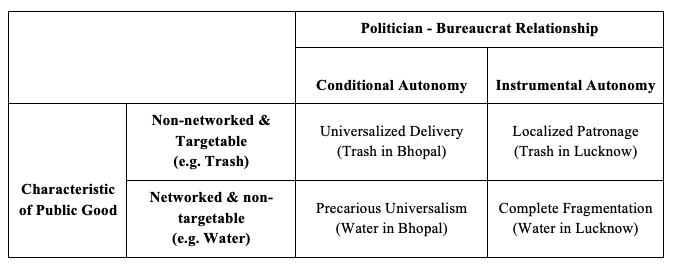
\includegraphics[width=.8\textwidth]{images/2by2new.png} % Adjust the width as needed
    \caption{Relationship between characteristic of Public Good and Politian-Bureaucrat Relationship}
   
\end{figure}

By highlighting conditional autonomy, this framework challenges the assumption that patronage and programmatic governance form a simple continuum. Patronage conditions do not preclude improvement. State-level bureaucrats, acting as intermediaries, can incrementally “upgrade” patronage systems by establishing professional norms, investing in capacity-building, and engaging politicians and contractors in strategic negotiations. In other words, conditional autonomy does not promise Weberian perfection, , but it can push systems toward more reliable and equitable service delivery than would be expected in a purely patronage-driven environment

The comparative cases of Bhopal and Lucknow illustrate these dynamics. Bhopal’s state-level bureaucrats secured a measure of conditional autonomy that facilitated citywide improvements in piped water access—albeit imperfect and precarious—while Lucknow’s collusive environment generated persistent fragmentation, stalled reforms, and reliance on informal arrangements. These empirical findings confirm that even in challenging political landscapes, conditional autonomy can help bureaucrats shepherd complex public goods projects closer to broad coverage and technical reliability.




\section{Institutional Paralysis \& Water Governance: The Case of Lucknow}

\subsection{Introduction}
The case of Lucknow vividly illustrates how institutional ambiguity and contested authority can obstruct coherent water service delivery. Here, the Jal Sansthan (LJS), formally tied to the municipal government but never truly integrated, occupies a precarious “\textit{Trishanku}-like” (twilight) state—nominally independent, yet effectively beholden to state-level agencies. As a result, each layer of authority pursued its own agenda, from state-level ministries resistant to local autonomy, to municipal officials constrained by financial instability, to LJS engineers lacking the power to implement technical solutions. Despite availability of finance and policy incentives, no credible intermediaries emerged to reconcile these divergent priorities. Instead of forging even minimal autonomy—such as localizing the Project Implementation Unit of a union government program or rationalizing water tariffs—politicians and bureaucrats gravitated toward short-term strategies, patronage-based arrangements, and fragmented service delivery. In theoretical terms, these dynamics align with the “collusion” scenario, where patronage politics and instrumentalized bureaucracies undermine attempts at structured, equitable solutions and trap institutions in persistent underperformance.


\subsection{Origins of Institutional Ambiguity: The Evolution of Lucknow City Water Utility}

\begin{quote} “Hum trishanku hai. Na idhar na udhar (We are in a twilight zone. Neither here nor there).”\footnote{Interview with the General Manager, Lucknow Jal Sansthan, Lucknow, 2022} 
\end{quote}

This was how the head of the Lucknow Jal Sansthan (LJS), Lucknow’s city-level water utility, described his institution’s predicament. Borrowed from a mythological king suspended between heaven and earth, the metaphor aptly conveys the LJS’s unsettled status.\footnote{In Hindu mythology, King Trishanku desired to enter heaven in his physical form. When the sage Vashishtha refused to help, Trishanku sought help from others, ultimately angering powerful figures and earning a curse. Attempts by Sage Vishwamitra to send him to heaven failed, leaving Trishanku suspended upside-down between earth and heaven. Determined, Vishwamitra created a new realm for him, and Trishanku remained there, eternally inverted. This tale birthed the phrase “Trishanku’s heaven,” denoting an unresolved, in-between state.} Formally tied to the city government yet never fully integrated, and nominally independent yet effectively beholden to external authorities, the LJS has failed to secure the operational coherence and autonomy envisioned when it was established in the mid-1970s. 

The Lucknow Jal Sansthan operates under a complex governance framework involving three distinct layers of control, each with its own priorities and limitations. (Figure 1):

At the highest level, the State Water Department maintains oversight through policy directives and funding decisions. However, with approximately 78\% of Uttar Pradesh's 241 million residents living in rural areas, the department's priorities and resources are heavily skewed toward rural needs. This imbalance is starkly reflected in the budget allocation: of the \$2 billion water budget, only \$241 million is designated for all urban utilities combined, with the remaining \$1.8 billion directed to rural areas. This distribution severely limits the resources available for urban infrastructure investment in cities like Lucknow.\footnote{PRS Legislative Research. (2021). \textit{Uttar Pradesh budget analysis 2021-22}. Retrieved from \url{https://prsindia.org/budgets/states/uttar-pradesh-budget-analysis-2021-22}} 

At the middle level, the Uttar Pradesh Jal Nigam (UPJN) serves as a parastatal authority responsible for technical standards, staffing decisions, and resource allocation across the state. As a body overseeing multiple urban centers, the UPJN treats Lucknow as just one of many clients, making it difficult to provide the focused attention and financial stability that the city's water utility requires.

At the local level, while the LJS is technically part of the Lucknow Municipal Corporation (LMC) following reforms implemented in 2009, this integration exists largely on paper. The LMC has limited real authority over the utility's financial or personnel matters. Although it theoretically has the power to set water tariffs, the LMC lacks the resources to fully incorporate LJS's operations. Further complicating this relationship, LJS staff members remain hesitant about deeper integration with the LMC, citing concerns about maintaining technical standards and stable payroll, particularly given the LMC's challenges in managing other services such as trash.

This tripartite arrangement leaves the LJS in a “Trishanku-like” state: formally linked to the city but effectively managed by higher-level bodies, financially dependent on state grants, and unable to carve out a coherent role for itself in local governance. To understand how these conditions emerged, we must examine the historical and structural choices that shaped Uttar Pradesh’s water governance institutions.

\begin{figure}[H] % Use [H] to force the image to appear exactly where you place it
    \centering
    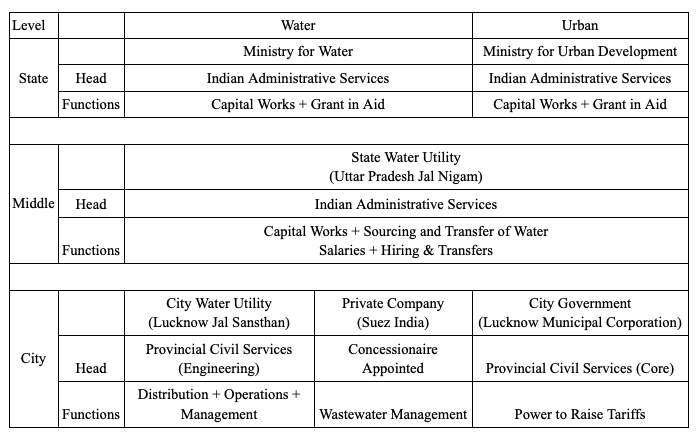
\includegraphics[width=1\textwidth]{images/Lwater.png} % Adjust the width as needed
    \caption{Administrative Institutions Governing Water Systems in Lucknow. Different Sources}
   
\end{figure}

Uttar Pradesh’s water sector modernization began in earnest in the 1970s, with international financial institutions—most notably the International Bank for Reconstruction and Development (IBRD), a precursor to the World Bank—offering funding and strategic guidance.\footnote{The Uttar Pradesh Water Supply and Sewerage Act, 1975 (Act 43 of 1975)}, Their core recommendation was to create specialized utilities capable of operating independently, raising their own revenues, and maintaining infrastructure without continuous state subsidies. Enacted in 1975, the Uttar Pradesh Water Supply and Sewerage Act established two new entities: the Uttar Pradesh Jal Nigam (UPJN) to oversee water management statewide, and city-level Jal Sansthans (including the LJS) to bring professional expertise and financial self-sufficiency to urban water provision.\footnote{During 1975–1990, the IBRD and the World Bank funded initiatives in “KAVAL towns” (Kanpur, Agra, Varanasi, Allahabad, and Lucknow) to test greater urban autonomy in water supply management.}

In theory, this arrangement promised a technical and managerial revolution. The Jal Sansthans were to operate like public utility companies, directed by expert general managers and supported by stable, tariff-based revenue streams. UPJN would coordinate larger projects and ensure statewide standards, while each Jal Sansthan would focus on local operations. In practice, however, these reforms never fully took root. Instead of forming distinct urban cadres or developing robust local revenue models, the Jal Sansthans remained administratively and financially tethered to UPJN and the State Water Department. Human resource reforms were neglected, and the same engineering cadres circulated among rural and urban postings, undermining the envisioned city-centric professionalism.\footnote{For a more detailed discussion read: India - Uttar Pradesh Water Supply and Sewerage Project (English). Washington, D.C. : World Bank Group. \protect\url{http://documents.worldbank.org/curated/en/979771468035977277/India-Uttar-Pradesh-Water-Supply-and-Sewerage-Project}}

\subsubsection{Persistent Rural Bias and Financial Constraints}

The skewed allocation of resources in Uttar Pradesh is crucial to understanding the LJS’s predicament. With 78\% of the population and pressing development needs located in rural areas, it is politically and administratively easier for state authorities to channel resources outside cities. This results in a systemic rural bias: rural sectors receive approximately \$9.62 per capita from the water budget, while urban residents must make do with about \$4.56 per capita.\footnote{PRS Legislative Research. (2021). \textit{Uttar Pradesh budget analysis 2021-22}. Retrieved from \url{https://prsindia.org/budgets/states/uttar-pradesh-budget-analysis-2021-22}} Although there may be developmental logic behind prioritizing rural areas—where farmers and low-income populations require immediate support—this imbalance starves urban utilities like the LJS of stable funding. Without adequate financial resources, LJS struggles to invest in trunk infrastructure or maintain existing networks, perpetuating weak service provision and low cost-recovery. The inability to generate sufficient revenue internally further cements its dependence on higher-level authorities.\footnote{See City Development Plan (pg. 18): \url{https://lmc.up.nic.in/pdf/nnfinal.pdf}; also World Bank South Asia Region Energy and Infrastructure Unit Report No. 27288 (2003).}

\subsubsection{Fragmented Staffing and Unstable Incentives}

The institutional complexity of Lucknow's water management system is deeply rooted in its workforce composition and leadership structure. The LJS and its parent organization, the Uttar Pradesh Jal Nigam (UPJN), are staffed by officers recruited through state-level engineering examinations. Senior officials come from the Combined State Engineering Services, while junior staff are selected through the Combined Junior Engineer Examination, collectively forming the Uttar Pradesh Engineering Services (UPES).

At the leadership level, the relationship between the UPES-cadre head of LJS and the UP Provincial Civil Services (UP-PCS) Commissioner of LMC has been marked by contention. Despite similar recruitment standards, these state officials operate under fundamentally different institutional frameworks. The UP-PCS officers manage broader administrative responsibilities and typically lead major state organizations like the LMC, while UPES officers maintain their specialized domain within water services, both in Lucknow and across the state.
The LMC's financial constraints also significantly influence this institutional relationship. From the LJS's perspective, deeper integration with the financially struggling LMC appears to offer little benefit while potentially adding bureaucratic complexity without improving their resource situation. Since funding and personnel transfers are managed at the state level rather than through Lucknow's municipal administration, the LJS has minimal incentive to subordinate itself to LMC oversight.

Field research reveals significant operational tensions, particularly among lower-level staff. Despite their formal subordination to the LMC, LJS employees strongly resist full integration, citing concerns about maintaining technical efficiency and professional autonomy(See figure 1.4). They frequently point to the LMC's challenges in managing solid waste—characterized by delayed salaries, procurement issues, and political interference in technical decisions—as a cautionary example of what might happen under complete municipal control.\footnote{Interview with the President, Uttar Pradesh Jalkal,Jalsansthan Adhikari/Karamchari Sanyukt Morcha, Lucknow 2021}
The state-wide transfer system for both engineering officers and staff creates additional complications. Many personnel prefer rural postings, which offer greater autonomy and control over resources, including more direct influence over infrastructure contracts and public works projects. In urban settings, these opportunities must be shared with the LMC, creating a less attractive professional environment. This preference for rural postings, combined with limited local institutional attachment and unclear advancement paths within the LJS, undermines staff commitment to addressing Lucknow's complex water management challenges.

\begin{figure}[H] % Use [H] to force the image to appear exactly where you place it
    \centering
    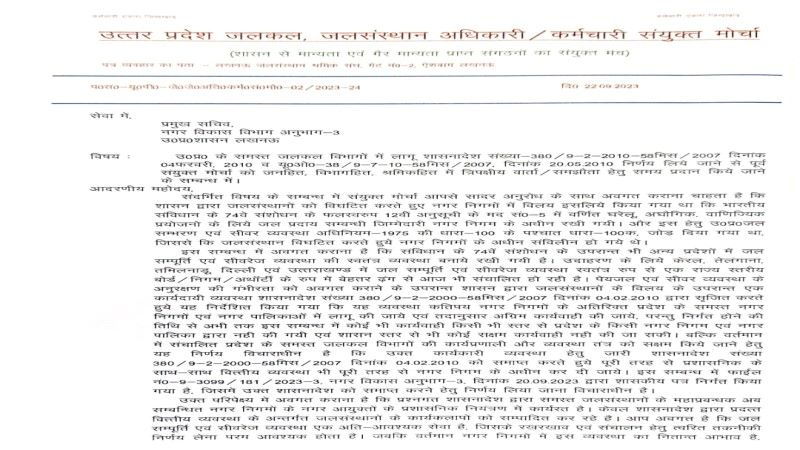
\includegraphics[width=1\textwidth]{images/पत्र-एक.jpg} % Adjust the width as needed
    \caption{Letter from the employee association against merger of the LJS with LMC, Lucknow 2023. Source: Primary Field Work}
   
\end{figure}

As a technically-oriented engineering organization, the LJS maintains a deliberate distance from political interfaces, operating through separate administrative offices distinct from the Lucknow Municipal Corporation's (LMC) facilities where political actors typically engage with municipal officials. While the LJS presents this separation as necessary to preserve technical autonomy and operational efficiency, this institutional arrangement has created problematic barriers to democratic accountability. The physical and organizational separation from political oversight has fostered an environment of bureaucratic insularity that diminishes responsiveness to public concerns. This disconnect is particularly evident in the experiences of elected officials within the LMC. These representatives, including municipal councilors, find themselves in an untenable position: they are the primary recipients of citizen grievances about water services yet lack effective mechanisms to influence LJS operations or demand improvements. As revealed in interviews, even the Mayor of Lucknow encounters significant difficulties in securing meetings with LJS officials, highlighting the extent of bureaucratic unresponsiveness.\footnote{Interview with Sanyukta Bhatia, Mayor of Lucknow Municipal Corporation from 2017-2023 }

The absence of robust oversight mechanisms and performance monitoring frameworks has allowed the LJS to operate with minimal public accountability. This institutional design, while potentially shielding technical operations from political interference, has ultimately contributed to persistent service delivery challenges that remain unaddressed due to the lack of effective channels for political and public oversight.

International agencies have tried to break these silos. External donors and consultants advocated for holistic reforms that would link water provisioning to broader urban development goals. For instance, they suggested using enhanced property tax revenues—administered by the LMC—to cross-subsidize water infrastructure managed by LJS. In theory, this approach could address LJS’s revenue shortfalls, reduce reliance on state grants, and foster greater integration between technical and administrative arms of the city. Yet these initiatives faltered. Each institution—UPJN, LJS, LMC—guarded its autonomy and prerogatives. Without a shared platform or credible enforcement mechanisms, negotiations stalled. The LMC lacked confidence in channeling scarce revenues into an entity it could not fully control, and LJS officers, mistrusting LMC’s fiscal instability, remained reluctant to recalibrate their internal procedures or accountability lines.
This persistent fragmentation prevented external interventions from catalyzing meaningful institutional change. Even when well-funded international programs offered opportunities for capacity-building and better financial planning, the entrenched patterns of isolation and resistance proved difficult to overcome. The LJS’s precarious position, lacking both proper autonomy and genuine integration, meant that it could not leverage external inputs effectively, and citywide strategies for improved service delivery remained unrealized.

In sum, the Lucknow Jal Sansthan’s enduring “Trishanku-like” condition emerges from a confluence of historical, institutional, and political factors. Intended as a technically autonomous utility, LJS instead became a hybrid entity, trapped among competing jurisdictions, weak revenue streams, and ambiguous lines of authority. The subsequent sections will show how this unsettled organizational landscape hinders coherent reforms, encouraging reliance on informal, short-term coping strategies rather than durable improvements in water delivery.




\subsection{Contested Authority: State Control versus Municipal Autonomy}

The institutional ambiguity and contested authority discussed above prevented Lucknow’s political and bureaucratic actors from reconciling their divergent priorities. As the city’s water challenges intensified, these misalignments solidified into persistent conflicts among state-level politicians, elite bureaucrats, and city-level officials in the LMC and LJS. Instead of devising a cohesive strategy, each faction pursued its own agenda, resulting in fragmented governance and inefficiency. Despite substantial external funding and reform incentives, such as those provided under JnNURM, these tensions meant that large-scale investments failed to produce lasting infrastructure improvements or reliable service delivery. Examining how these elite-level coordination failures shaped the water utility’s capacity thus illuminates the everyday realities of water access in Lucknow.

\subsubsection{\textbf{Differing Perspectives Among Stakeholders}
}
Elite state-level bureaucrats, particularly those in the Indian Administrative Service (IAS), consistently portrayed water as a foundational public good best managed through technical standards and centralized authority. One former Secretary of Water Resources emphasized the importance of professional insulation:

\begin{quote} "The real obstacle is not the availability of water—Uttar Pradesh has more than enough sources—but the inability to implement solutions free from local meddling. When every decision is subject to neighborhood-level demands and short-term political interests, you lose technical rigor and long-term vision. Keeping the system under state-level control ensures that engineering standards, not local pressures, guide the process. Only then can we achieve true efficiency and competence."\footnote{Interview with the Secretary, Department of Water Resources (2012-2018), Indian Administrative Services. Lucknow}
\end{quote}

For these technocrats, Uttar Pradesh’s abundant water was not scarce, but poorly managed. Insulating water governance from local political bargaining and relying on professional engineering cadres, in their view, provided the clearest path to maintaining quality, reliability, and fairness.

State-level politicians, however, often adopted an even more radical stance that rejected the commodification of water. Former Urban Development Minister Mohd. Azam Khan publicly opposed installing water meters—a measure intended to improve cost recovery and operational efficiency. In an interview, he justified this position

\begin{quote} “We have enough water. They [bureaucrats] used to tell me water rates needed to be increased… new meters need to be installed. I said use these funds to improve the drinking water supply infrastructure. People use water only as much as they need. They don’t waste any water. Actually, you are the ones who lose water.. Half of the water in Lucknow is lost during transmission. Surely, this is not people’s fault.”\footnote{Interview with Md. Azam Khan, Minister for Urban Development (2012-2017), Rampur Jail 2022.}

\end{quote}

While the minister acknowledged that low per capita incomes might limit consumers’ ability to pay, the primary critique targeted systemic inefficiencies—distribution losses, poor infrastructure, and unreliable quality—rather than consumer behavior. Official reports indicate that operational losses—primarily due to leakage, inefficient maintenance, and outdated infrastructure—consistently hover around 50\%, underscoring the entrenched inefficiencies that persist despite decades of policy interventions and attempted reforms (See table 1.2). Notably though, this stance was not mere electoral expediency; it represented a deeper ideological position on public service provision. Another Minister for Water Resources echoed similar sentiments, reflecting a stable ideological position rather than mere electoral pandering.\footnote{Same sentiment was repeated by Ashoka Kumar Dohre, Minister for Water Resources (2007-2011). Lucknow 2022, 2023.} For these state politicians, water was a non-negotiable right, and any talk of pricing or metering threatened to politicize the issue and alienate voters.

At the city level, however, the LMC—home to city bureaucrats and municipal politicians—saw matters differently. Municipal officials argued that local control over water utilities could improve responsiveness. “If we had them [LJS under LMC control], we would understand the city’s needs and serve more effectively,” explained one LMC Commissioner.\footnote{Interview with Commissioner, Lucknow Municipal Corporation (2022), UP Provincial Civil Services, Lucknow 2022} City-level politicians like municipal councilors also stressed that LJS engineers focused on technical parameters while ignoring the everyday realities of informal neighborhoods. “They do surveys and make estimates. We know the ground realities—our ears are to the ground, theirs are in the Secretariat,” lamented a former councilor.\footnote{Interview with Md. Saifullah, Councillor (2012-2017), Lucknow 2022} Yet city-level politicians and administrators recognized a harsh truth: the LMC lacked the financial muscle to absorb LJS fully. The former Mayor, Dinesh Sharma, conceded, “We simply do not have the funds to pay LJS employees… unless the state keeps providing grants.”\footnote{Interview with Dinesh Singh Sharma, Mayor (2006-2017), Minister for Urban Development (2017-2022), Lucknow 2021} 

Within the LJS itself, engineers and managers resented both local political meddling and the constraints imposed by state authorities. As one General Manager, the head of LJS explained:

\begin{quote}

 “We are stuck in a cycle: without adequate revenue, we cannot invest in infrastructure; without improved infrastructure, residents will not trust us enough to pay. Every time we try to break this loop—say, by proposing a tariff increase—either the state pushes back or local politicians object. It’s not that we don’t understand what needs to be done. We do. But without the authority to set rates, hire qualified staff, or control our own budgets, we’re forced to patch things up with short-term fixes. This isn’t about engineering anymore.”\footnote{Interview with General Manager, Lucknow Jal Sansthan (2013-2016). Lucknow 2023}\end{quote}

Their perspective was that without proper revenue mechanisms—such as rationalized tariffs and widespread metering—to generate the funds needed for infrastructure upgrades, the cycle of underinvestment, poor quality, and low trust would remain unbroken.

These divergent perspectives—state-level politicians wary of metering, top bureaucrats favoring centralized technical control, city officials seeking greater local authority, and LJS engineers advocating for revenue-generating mechanisms like metering—would not necessarily doom reform if credible intermediaries existed to align their interests. In many settings, political leaders or bureaucrats step forward to translate high-level mandates into workable arrangements; in others, civil society organizations outside the state persuade key actors to act. In Lucknow, however, such intermediation never materialized.

\begin{table}[h!]
\centering
\caption{Water Supply and Losses (2005-2019)}
\begin{tabular}{|p{1.5cm}|p{2.5cm}|p{2.5cm}|p{2cm}|p{3cm}|p{2.5cm}|}
\hline
\textbf{Year} & \textbf{River Water (MLD)} & \textbf{Ground (MLD)} & \textbf{Total (MLD)} & \textbf{HH with piped water (\%)} & \textbf{Losses (\%)} \\ \hline
2005 & 270 & 190 & 205 & 47\% & 53\% \\ \hline
2016 & 475 & 400 & 875 & 62\% & 30\% \\ \hline
2019 & 400 & 630 & 756 & 64\% & 45-50\% \\ \hline
\end{tabular}
\caption*{Source: City Development Plan, pg. 19-20. All figures supplied by Lucknow Jal Sansthan.}
\end{table}


A telling example comes from the scenario described by a civil society representative who observed the union government's program (Jawaharlalal Nehru National Urban Renewal Mission or JnNURM) implementation in Uttar Pradesh.\footnote{Under JnNURM: central government typically contributed 50\% of project costs, the state government 30\%, and the
city government 20\%. State and city governments often relied on organizations like the ADB, World Bank, DFID, or
USAID for their shares.} Each grant-receiving city was paired with an international agency offering capacity-building support—specialized consultants in human resources, finance, and governance—at no cost.\footnote{ For Lucknow this agency was US-AID which funded this project under the Financial Institutions Reform and Expansion–Debt and Infrastructure (FIRE-D)} The arrangement was intended to last the full duration of the ten-year funding period, a substantial opportunity for institutional strengthening. In mid-2007, as discussions arose over the placement of the Project Implementation Units (PIUs), as these capacity building offices were referred to, the city’s Municipal Commissioner proposed situating the PIU within local agencies. The Commissioner argued that doing so would improve coordination, allow responsive adjustments, and ensure that technical expertise guided daily operations. LJS officials also supported embedding consultants in their departments.

Yet, as the civil society representative recalled, the idea of placing the PIU in either the LMC or LJS was never seriously entertained. “Cities in UP were complete pushovers,”\footnote{Interview with the Member from Regional Center for Economic and Urban Studies, Lucknow. Lucknow 2021, 2022} she explained. “Secretaries would say, ‘Lucknow does one thing—garbage. They don’t need consultants for that.’” When she countered that the city’s limited capacity was precisely why the PIU was needed on-site, a senior bureaucrat offered a further rationale: “If Lucknow got the PIU, other cities would soon demand the same. We ourselves were starved of talent. In 2005, I had two computer operators for over five hundred urban local bodies. The hope was that centralizing expertise would eventually trickle down.” In the end, the PIUs were set up at the state secretariat (rebranded as Project Management Units or PMU). Over time, as fresh funding arrived in 2009, and again in 2011 and 2016, the question of relocating PIUs to the city reemerged, only to be rebuffed each time.

The inability of the LMC and LJS to secure the relocation of the PIU from state-level agencies to the city underscores the depth of their institutional constraints. Despite the PIU representing a relatively modest administrative reform, neither the LJS nor the LMC could successfully advocate for its placement within their organizations. This failure to secure even this small measure of autonomy revealed the extent of their institutional isolation and debilitation.

The state's refusal to relocate the PIU pointed to a more fundamental governance crisis. Lucknow's city-level bureaucrats found themselves in an impossible position: nominally responsible for water service delivery yet lacking the basic tools of administrative authority. While they had gained certain peripheral powers, such as tariff-setting authority, the state retained iron grip over all meaningful levers of control - staffing decisions, capital budgeting, and procurement authority. This arrangement left city officials unable to build the institutional credibility needed to advocate for greater autonomy.

The circular nature of this predicament proved particularly damaging. Without a track record of successful administration, city bureaucrats could not convince state authorities that localizing the PIU would enhance project governance. Yet without control over basic administrative functions, they could not develop the capabilities and safeguards that might have demonstrated their readiness for greater responsibility. State officials could always point to this lack of proven capacity to justify maintaining centralized control, perpetuating a cycle of institutional weakness that made meaningful reform increasingly difficult.

\subsubsection{Failed Reform and Institutional Stalemate}

This dynamic of mutual mistrust and restricted authority did not remain a theoretical concern; it materialized in the city’s encounters with national and international development programs. As discussed earlier, the PIU instead of operating locally, embedding specialized consultants in the LMC and LJS was placed in the Secretariat. These arrangements—tolerated by international agencies despite violating original contract terms—led to delays and growing dissatisfaction. Consultants noted that senior bureaucrats in Lucknow insisted the Secretariat (by which they meant the State government) was the only suitable locus of control.\footnote{Interview with RK Srinivasan, USAID Water, Sanitation and Hygiene Finance (WASH-FIN) Delhi 2023} Yet by excluding local politicians and the LJS from meaningful input, the state created a knowledge vacuum. Without LJS insights, critical decisions—such as whether to pursue comprehensive city-wide coverage or focus first on established urban cores—became contentious. The state-level utility favored newly incorporated areas like Gomti Nagar and Transport Nagar, anticipating modernization and better returns through user fee, while the LMC advocated improvements in older neighborhoods aligned with its political base.\footnote{Interview with Fire-D consultants in PMU Lucknow 2009-2012, Delhi 2023} The resultant stalemate was not merely technical but deeply political, revealing the institutional fault lines embedded in Lucknow’s water governance. In this, the LJS - the body which actually had to do the work had little or no say. 

The politicization of procurement compounded the problem. With the ruling Samajwadi Party favoring a Dubai-based firm and the BJP-led municipal government insisting on the lowest bidder, contractor selection controversies escalated.\footnote{Interview with SK Singh, PCS officer, Commissioner of Lucknow 2007-2012. Delhi 2023} Allegations surfaced that BJP leaders privately lobbied for companies tied to their party, including one owned by the son of a then-Member of Parliament.\footnote{ibid.}Such politicization and marginalization of local expertise eroded confidence in the reforms, and ultimately led to key international agencies reducing or withdrawing their support. Independent evaluators offered harsh assessments:

“In Uttar Pradesh, stakeholders noted very low capacity across the state and perennial recruitment challenges further complicated by the state government’s fragmented management and shifting directivess. Capacity to plan and execute development projects is weak, and Lucknow’s low-level staff capacity to manage finances and technology is limited. Although a state-run utility is functioning, it is not always timely or geared to meet the on ground implementation challenges.” \footnote{India Financial Institutions Reform and Expansion–Debt and Infrastructure Ex-Post Evaluation, WASH Ex-Post Evaluation Series—Water Communications and Knowledge Management (CKM) Project, September 2018.}

In short, the FIRE-D episode underscores how the city’s lack of autonomy, combined with deep-seated political and bureaucratic tensions, neutralized opportunities for meaningful institutional strengthening. The very tools designed to foster local capacity and guide incremental reform became instruments of centralization, reinforcing a status quo in which neither efficiency nor accountability could flourish. Instead of bridging the gap between grand policy visions and street-level implementation, these international interventions remained stranded at the top, divorced from the local knowledge and authority needed to translate reforms into tangible improvements.

This same pattern of misalignment and inertia manifested itself in another key arena: the debates over water pricing policy. Since the early 2000s, city-level politicians, engineers, and select bureaucrats had recognized that static or token-level water tariffs could not sustain investments in infrastructure, maintenance, and service improvements. Although formal records indicate multiple resolutions passed by the Lucknow Municipal Corporation (LMC) to rationalize water rates—most recently in 2019—these attempts consistently stalled.\footnote{Proceedings of the Lucknow Municipal Corporation. Accessed from the Archives of the Lucknow Nagar Nigam Record Room. Lucknow 2021,2023} The rationale for pushing new tariffs was simple: marginalized groups in informal settlements were already paying private suppliers at higher rates for unreliable service. If the city could guarantee better quality and more dependable supply, many residents, even the poor, might accept moderate user fees.\footnote{ibid}\footnote{Interview with Syed Yawar Hussain Reshu, Leader of the Opposition, Lucknow city corporation, Lucknow 2022}

Yet, as city officials weighed these options, they confronted an entrenched resistance at the state level. State level politicians opposed both tariff hikes and the introduction of metering. Even senior bureaucrats in the Water Ministry framed metering and tariffs as distractions from addressing deeper structural issues: massive leakages, deteriorating pipelines, and haphazard distribution networks. Rather than turning to pricing mechanisms, these state-level actors urged the LJS to improve operations first—a proposition that seemed paradoxical, since operational improvements required stable revenue streams the LJS did not have. Interviews with senior bureaucrats shed further light on this impasse. Even sympathetic IAS officers, who privately acknowledged the necessity of pricing reforms, found it impossible to shift political positions. As one IAS officer who served in multiple state departments recounted:

 \begin{quote}

 “We tried to make a case to the Minister, but we had pumped so much money under various schemes and nothing really improved on the fiscal side, so it was tough to convince anybody on issues of water tariff.”\footnote{Interview with IAS officer who served in Water, Finance, Rural and Urban Development Ministry and retired as Additional Chief Secretary, Government of Uttar Pradesh. Delhi and Lucknow 2021-2024} \end{quote}

In other words, earlier failures to produce tangible improvements had eroded the credibility of reform advocates. Without visible results to justify higher charges, political leaders feared public backlash and questioned why consumers should pay more for the same unreliable service. This climate of mistrust and reluctance to invest political capital in unpopular decisions undercut any hope of implementing rational tariffs.

Caught in the middle, the LJS struggled to reconcile these opposing pressures. Local officials understood that without adjusting tariffs and introducing metering, the utility would remain trapped in a cycle of poor revenue generation and underinvestment.

Despite this clarity, the proposed compromise—municipal funding for meters combined with state-financed capital works—collapsed under fundamental fiscal constraints. Limited pilot attempts to install meters in newer neighborhoods yielded negligible results, not only due to technical shortcomings but also because consumers had grown accustomed to flat rates and informal arrangements. By 2019, official reports showed that citywide metering remained a distant goal.\footnote{Office of the Principal Accountant General (General \& Social Sector Audit), Uttar Pradesh. (2016). Annual Technical Inspection Report on Urban Local Bodies for the Year Ended 31 March 2016 (p. 23, 24). Government of Uttar Pradesh.} Without usage-based billing or cost-reflective tariffs, operational costs continued to outstrip revenues, perpetuating dependence on state subsidies and informal coping strategies.

Compounding these fiscal challenges, corruption and inefficiencies in billing and collection practices eroded the system’s integrity. State audits, newspaper investigations, and vigilante raids by the state’s Vigilance Department uncovered patterns of underreported water usage, unauthorized amnesties granted to favored consumers, and the deliberate undervaluation of property sizes in affluent neighborhoods.\footnote{During fieldwork, it was observed that frequent allegations of bribery and “overlooking” large connections were reported in local dailies. The state’s Vigilance Department also conducted raids, uncovering assets of top LJS officials vastly disproportionate to their incomes. In one noted case, a UP Jal Nigam employee possessed assets worth over \$4.8 million USD, far exceeding legitimate earnings.}

These malpractices illuminated the perverse incentives sustaining the status quo. Local politicians sometimes colluded with LJS field officers to supply discounted tanker water to informal settlements in exchange for under-the-table payments. Such arrangements, while offering short-term relief, entrenched patronage networks and discouraged systematic reforms. Both LJS staff and municipal officials privately acknowledged these informal workarounds as a symptom of a governance environment dominated by immediate political pressures rather than long-term strategic planning.

These governance fractures and political deadlocks carried significant fiscal consequences. Without rationalized tariffs or effective metering, the LJS forewent substantial revenue (estimated around  \$40.1 million) due to its inability to secure effective local management structures and coherent intermediation that could have financed infrastructural improvements and operational reforms. Earlier coordination failures, including missteps in project site selection and the failure to integrate external capacity-building measures, had already diminished the city’s access to critical development funding. An independent end-of-project appraisal underscored the gravity of these shortcomings: “No studies have been undertaken to assess the impact of subsidies on water supply, sewerage, and waste management services. Coverage remains at only 62\%, and bulk meters at source and distribution points are yet to be installed. Interdepartmental coordination between Jal Nigam, Jalkal, and LNN remains weak, hampering service quality and the feasibility of user charges. Full integration and a formal inter-governmental mechanism for coordination are still lacking.”\footnote{CRISIL Risk and Infrastructure Solutions Limited. (2014). \textit{Reform Appraisal Report – UIG: Uttar Pradesh – Package 3}. Mission Directorate, Jawaharlal Nehru National Urban Renewal Mission (JNNURM), Ministry of Urban Development. Retrieved from \url{https://localbodies.up.nic.in/CRISIL\%20REPORTS/UIG.pdf}, p. 73.}

In theory, JnNURM-linked reforms and legislative amendments should have broadened local autonomy and improved institutional coherence. Instead, they produced what organizational theorists term “myths and ceremonies” \citep{meyer_institutionalized_1977}—formal compliance with reform conditions, but scant substantive change. This disconnect became starkly evident in two critical arenas: the placement and operation of externally funded capacity-building programs, and efforts to rationalize water tariffs.

As a result, international agencies’ stipulations for a city-level PIU were met only in form, not in substance, and the intended capacity-building benefits never materialized. These arrangements—tolerated by international donors despite violating original contract terms—led to delays and mounting dissatisfaction. Consultants noted that senior bureaucrats in Lucknow insisted the Secretariat was the only suitable place for control.\footnote{Interview with RK Srinivasan, USAID Water, Sanitation and Hygiene Finance (WASH-FIN) Delhi 2023} Yet excluding local politicians and the LJS from meaningful input created a knowledge vacuum. Without the LJS’s insights, critical decisions—such as whether to target comprehensive citywide coverage or begin with established urban cores—were contentious. The state-level utility favored newly incorporated areas like Gomti Nagar and Transport Nagar, anticipating modernization and better returns through user fees, while the LMC pressed for improvements in older neighborhoods aligned with its political base.\footnote{Interview with FIRE-D consultants in PIU Lucknow 2009-2012, Delhi 2023} This stalemate was not merely technical but deeply political, revealing the institutional fault lines embedded in Lucknow’s water governance. Throughout this process, the LJS—the entity ultimately responsible for carrying out the work—was relegated to the sidelines, its expertise and local knowledge overshadowed by top-down dictates.

Procurement politicization further complicated the reforms. With the ruling Samajwadi Party favoring a Dubai-based firm and the BJP-led municipal government insisting on the lowest bidder, contractor selection controversies escalated.\footnote{Interview with SK Singh, PCS officer, Commissioner of Lucknow 2007-2012. Delhi 2023} Allegations soon surfaced that BJP leaders privately lobbied for companies tied to their party, including one owned by the son of a then-Member of Parliament.\footnote{ibid.} Such politicization fueled mistrust, undermining the credibility of reforms. The minister overseeing the project (currently serving jail time on corruption charges related to these initiatives)\footnote{Jal Nigam recruitment scam: \textbackslash{}url\{https://hindi.news18.com/news/uttar-pradesh/lucknow-jal-nigam-recruitment-scam-sit-submits-report-seeks-permission-to-register-fir-against-azam-khan-1355416.html} openly dismissed international partners, telling me:

\begin{quote} “The international partners were not important; they put undue pressure to bring their own people and agencies, but we did not think that way.” \end{quote}

This cavalier attitude eroded confidence and magnified doubts about the reforms’ integrity. Ultimately, misaligned incentives, political meddling, and institutional skepticism prompted key international agencies to withdraw support. The World Bank halved its commitment; USAID’s FIRE-D program also exited after disagreements over project direction.\footnote{Interview with RK Srinivasan, USAID Water, Sanitation and Hygiene Finance (WASH-FIN) Delhi 2023} In the project evaluation reports, independent auditors offered harsh assessments:

\begin{quote} “In Uttar Pradesh, stakeholders noted very low capacity across the state and perennial recruitment challenges further complicated by the state government’s fragmented management and shifting directives. Capacity to plan and execute development projects is weak, and Lucknow’s low-level staff capacity to manage finances and technology is limited. Although a state-run utility is functioning, it is not always timely or geared to meet on-the-ground implementation challenges.”\footnote{India Financial Institutions Reform and Expansion–Debt and Infrastructure Ex-Post Evaluation, WASH Ex-Post Evaluation Series—Water Communications and Knowledge Management (CKM) Project, September 2018.} \end{quote}

Nominal reforms and promised international funding—intended to bolster local capacity and professionalize the LJS—therefore yielded scant results. Instead of enabling conditional autonomy or cultivating a capable local bureaucracy, the PIU arrangement became a top-down tool reinforcing state-level dominance. Centralized decision-making and entrenched mistrust neutralized external expertise and stifled long-term planning. Without clearly defined authority lines between state and municipal actors, Lucknow’s water governance remained an institutional void, offering neither the efficiency gains of a more autonomous bureaucracy nor the accountability of genuinely devolved authority.

To summarize, In the first section, the analysis focused on how the Lucknow Jal Sansthan (LJS) found itself trapped in institutional limbo—formally anchored to the city government but never truly integrated, and ostensibly under state authority yet lacking genuine autonomy. In this subsequent exploration of elite coordination failures, it became clear that neither city-level actors nor their state-level counterparts could overcome the deep-rooted mistrust and entrenched interests that thwarted effective policy implementation. Despite considerable external funding and policy incentives, no credible intermediaries emerged to reconcile divergent priorities and to build a more coherent governance structure. Instead of securing even modest autonomy—such as locating the PIU at the municipal level—or rallying behind incremental reforms like tariff adjustments, the city’s politicians and bureaucrats resorted to short-term political strategies and patronage, while state bureaucrats and politicians refused to relinquish meaningful control. This dynamic encapsulates what the theoretical framework characterizes as “collusion,” wherein patronage politics and instrumentalized bureaucracies lock institutions into a cycle of fragmentation and underperformance, ultimately denying the city and its residents the potential gains of more efficient, equitable, and sustainable water service delivery.


\subsection{ Emergence of Hybrid Solutions: Local Adaptations and Their Consequences}

The previous section illustrated how elite-level efforts to coordinate Lucknow’s water governance fell short, with state and city authorities locked in distrust and fragmented policymaking. Yet the demand for water did not simply evaporate. Under conditions of top-level fragmentation, local-level actors—frontline LJS staff, councilors, petty contractors, and neighborhood intermediaries—stepped in, relying on borewells, handpumps, and tubewells to fill service gaps. My field observations and interviews indicate that these stakeholders felt compelled to provide some tangible relief, however improvised or ad hoc. Rather than delivering stable, inclusive solutions, however, this bottom-up improvisation took the form of collusion—tacit, informal agreements that perpetuated selective gains, entrenched inequalities, and ultimately mirrored the very dysfunctions that plagued coordination at higher levels.



Despite official claims of increased coverage, a persistent gap remained. Various sources offered differing statistics: a 2019 government report suggested 62\% piped access, the LJS later claimed 80\% by 2022, but a citizen survey conducted co-terminus with this dissertation found only 72\% reported access (Table 1.3). Regardless of the exact figure, about 25–30\% of Lucknow’s population still lacked formal piped water. This widespread reliance on borewells, handpumps, and private arrangements—even among wealthier colonies—revealed a city-wide pattern:  even those with resources and political connections found it necessary to circumvent formal systems (Table 1.4). The absence of elite-level agreement had thus pushed the burden of ensuring basic access down to the local scale.

\begin{table}[ht]
\centering
\renewcommand{\arraystretch}{1.5} % Adjust row height
\setlength{\tabcolsep}{8pt} % Adjust column spacing
\begin{tabular}{|p{5cm}|c|c|}
\hline
\textbf{Source of Water} & \textbf{Bhopal (\%)} & \textbf{Lucknow (\%)} \\ \hline
Tap (Piped) & 86.11 & 72 \\ \hline
Borewell + Hand pump & 12 & 26 \\ \hline
Other sources & 2 & 2 \\ \hline
\multicolumn{3}{l}{\textit{Source: Primary survey under the Brown - India Citizenship Project 2022}} \\ % Add source note
\end{tabular}
\caption{Source of Water by City}
\label{tab:water_sources}
\end{table}

\begin{table}[ht]
\centering
\renewcommand{\arraystretch}{1.3} % Adjust row height
\setlength{\tabcolsep}{5pt} % Adjust column spacing
\begin{tabular}{|p{3cm}|p{3cm}|p{2.5cm}|p{3cm}|p{3cm}|}
\hline
\textbf{City} & \textbf{Housing Type} & \textbf{Tap (Piped)} (\%) & \textbf{Borewell + Hand Pump} (\%) & \textbf{Other Sources} (\%) \\ \hline
Bhopal & Shack          & 93 & 1  & 6  \\ \hline
       & Slum           & 97 & 2  & 1  \\ \cline{2-5}
       & Middle Class    & 87 & 12 & 1  \\ \cline{2-5}
       & Upper Middle    & 82 & 15 & 3  \\ \cline{2-5}
       & Rich            & 80 & 20 & 0  \\ \hline
Lucknow & Shack         & 48 & 37 & 15 \\ \hline
        & Slum          & 64 & 32 & 4  \\ \cline{2-5}
        & Middle Class   & 74 & 25 & 1  \\ \cline{2-5}
        & Upper Middle   & 71 & 29 & 0  \\ \cline{2-5}
        & Rich           & 78 & 21 & 1  \\ \hline
\multicolumn{5}{l}{\textit{Source: Primary survey under the Brown - India Citizenship Project 2022}} \\ % Add source note
\end{tabular}

\caption{Source of Water by City and Housing Type}
\label{tab:water_by_housing}
\end{table}

\vspace{2mm}


Groundwater extraction became the cornerstone of Lucknow’s de facto supply system (Table 1.5). The LJS maintained some 720 borewells, accounting for 25\% of the city’s groundwater draw, but a staggering one hundred fifty thousand (1.5 lakhs) privately managed wells contributed another 36\%.\citep{foster_lucknow_2009} Together, this decentralized infrastructure accounted for 99\% of total water extraction. This “solution” came at a high environmental and public health cost: the city earned an “over-exploited” classification for groundwater, and quality analyses frequently detected fluoride, arsenic, and fecal coliform contamination \citep{sinha_state_2021}.


\begin{table}[h!]
\centering
\caption{Groundwater Extraction in Lucknow}
\begin{tabular}{|p{4.5cm}|p{3cm}|p{4cm}|}
\hline
\textbf{Institution} & \textbf{Tube/Bore Wells (Units)} & \textbf{Tentative Ground Water Extraction (MLD)} \\ \hline
Lucknow Jal Sansthan (Borewells) & 720 & 356 \\ \hline
Private (Borewells, Tubewells, Handpumps, Submersibles) & 150,930 & 510 \\ \hline
Others & 640 & 533 \\ \hline
\textbf{Total} & \textbf{152,290} & \textbf{1,399} \\ \hline
\end{tabular}
\caption*{Source: Lucknow Jal Sansthan as mentioned in \citep{sinha_state_2021} }
\end{table}

As my fieldwork in Transport Nagar illustrates, informal settlements evolving on the city’s periphery navigated a dense web of political patronage and makeshift engineering. In informal settlements like Gindan Khera or Amausi, which emerged amid rapid urbanization and airport expansion, such hybrid provisioning became a necessity.\footnote{In Lucknow, the legality of a neighborhood significantly impacts residents' access to water services. However, this relationship is not a simple binary, as the type and location of the neighborhood also play a critical role. Illegal colonies near formal neighborhoods, particularly in the city's core, often have access to water connections due to a "spillover" effect. In contrast, residents of informal settlements like Transport Nagar rely on personal connections to local politicians or bureaucrats to secure water access. Obtaining a water connection is complicated by the fact that the Lucknow Municipal Corporation (LMC) grants No Objection Certificates (NOCs) for water, while the Lucknow Development Authority (LDA) determines land legality. This disconnect allows for discretion in granting NOCs, favoring those with the right connections. In affluent areas like Gomti Nagar, even residents of LDA-designated illegal colonies rarely face barriers to water access, unlike in Transport Nagar, where personal networks are more decisive. The complex interplay of legal, spatial, and social factors in shaping water access in Lucknow necessitates a nuanced understanding of water governance and citizenship that goes beyond simple binaries of legal/illegal and served/unserved.} Initially reliant on scattered hand pumps or distant public taps, these communities found that as the water table fell in the 1990s, a single tubewell managed by a local politician’s associates only partially eased the crisis. Soon, multiple private tubewells sprang up, charging residents INR 150–200 per month for thrice-weekly supply.\footnote{Field interviews, 2021,2022 }As the city densified, local MLAs and councilors leveraged their influence to install government-funded borewells or negotiate tanker deliveries. The result was a deeply politicized patchwork where gaining access often depended on personal connections, bribes, or being part of the councillors core support base. This qualitative finding is further reflected in the primary survey, which is representative of the city-level conditions in Bhopal and Lucknow (n=3,754). A full treatment of this is provided in Chapter 2, where I demonstrate empirically that knowing a politician personally increases the likelihood of receiving water services in Lucknow by 88.2 percentage points. This finding underscores that access to essential services is not merely anecdotal but systematically tied to political connections, as evidenced at the pan-city level. (See annexure for discussion of the key findings from the survey).

In Gindan Khera, for example, residents I interviewed described lining up for water from a community standpost only once or twice a week. When supply finally arrived—frequently at unpredictable hours, sometimes at dawn—they rushed to fill buckets and containers as quickly as possible. Those without personal connections to the local councilor’s aide or the borewell manager found themselves waiting longer or receiving less. Some residents admitted paying small “gifts” to the pradhan or the local party worker to secure water, particularly during the summer month and monsoon when ground water dried up or was laden with silt and impurities. One woman lamented, “If you don’t show your face at the councilor’s office or keep good relations with the pump operator, your household might end up with less water that week.” Another resident noted that wealthier neighbors sometimes negotiated private tanker deliveries, leaving poorer households to scramble for whatever trickled down. This was water access through informal patronage, not a stable public service.


\begin{figure}[H] % Use [H] to force the image to appear exactly where you place it
    \centering
    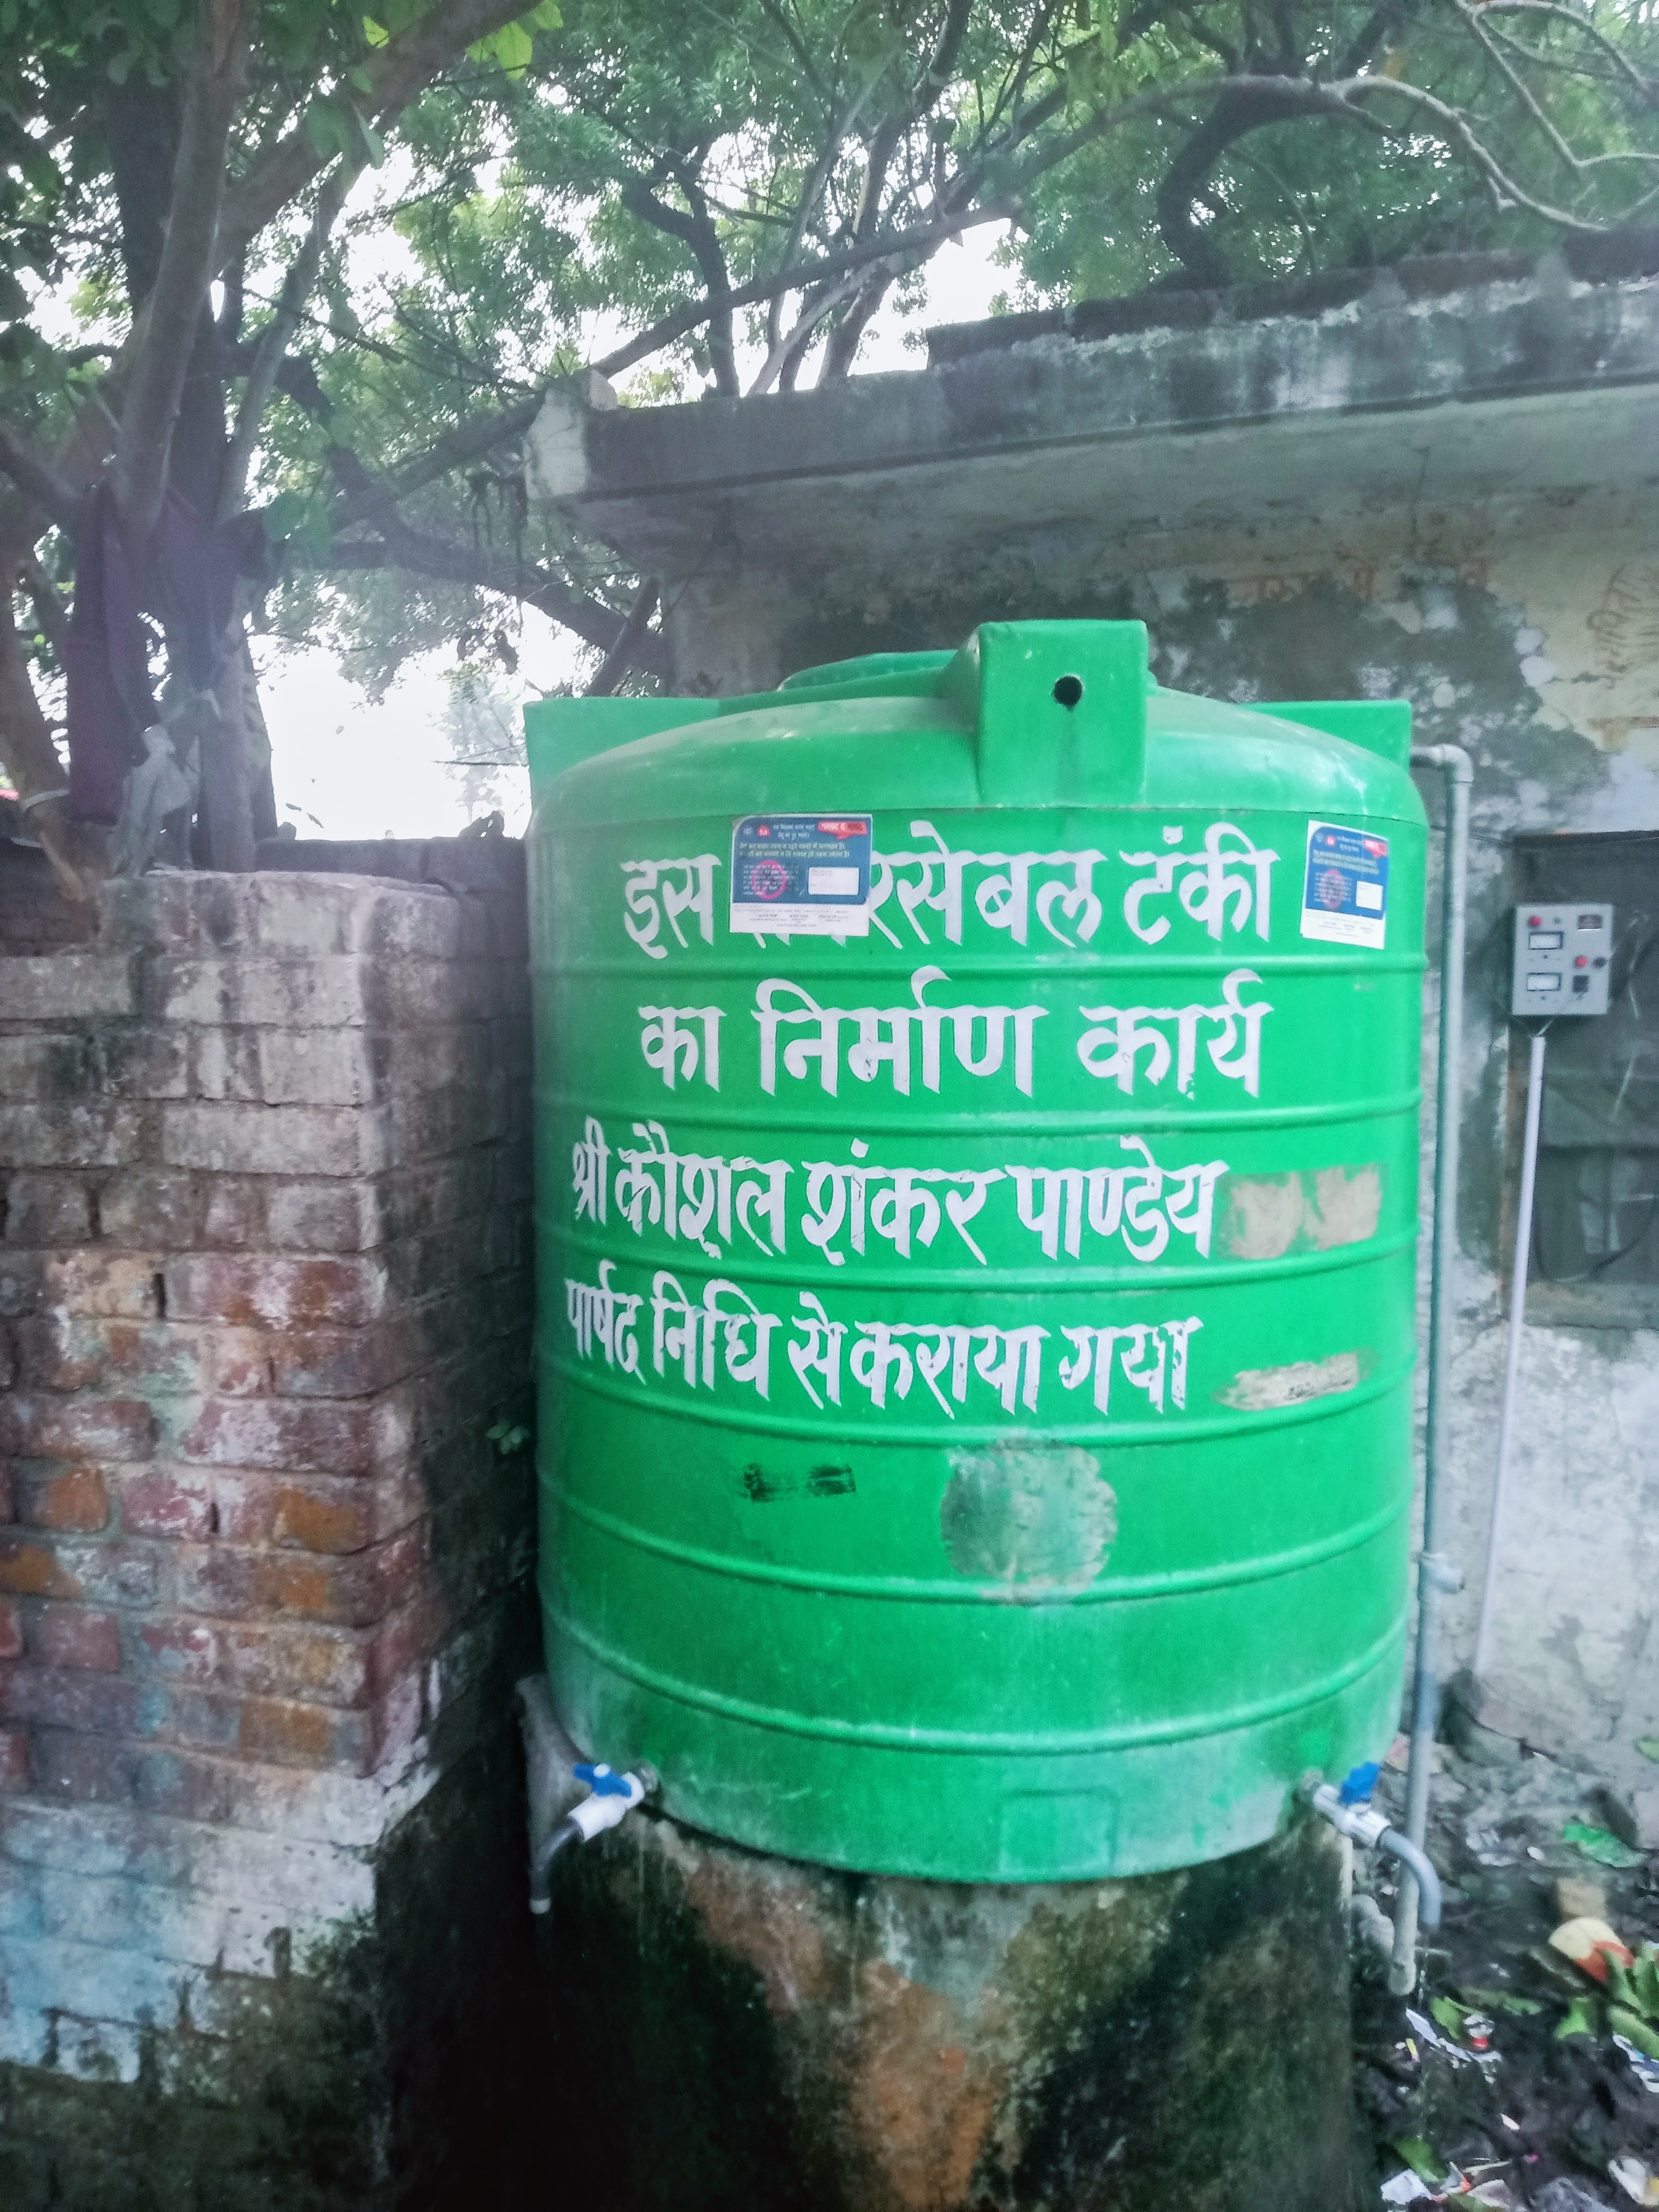
\includegraphics[width=.5\textwidth]{images/2by2.jpg} % Adjust the width as needed
    \caption{A submersible pump and tank installed by the ward councilor in Gindan Khera. Lucknow 2022}
   
\end{figure}


Securing even a single tubewell underscored the intricate coordination required at the grassroots level. Councilors responding to constituent demands petitioned the LJS for technical approvals and tendering, while the LMC, managing finances, often tapped councilors’ development funds and its own limited budget. The Sub-District Magistrate provided legal and administrative oversight.\footnote{Interview with LJS and Ward Councillors of Lucknow Municipal Corporation, Lucknow  2021 2022.} Within these negotiations, the LJS prioritized engineering standards and tendering, the LMC struggled to allocate scarce financial resources effectively, and councilors leveraged political influence to determine tubewell locations and managers. Installation costs ranged from INR 2.8 to INR 3.3 lakh, requiring multiple funding sources. \footnote{Interview with officials from the Public Health and Engineering Department, Government of Uttar Pradesh, Lucknow 2022}Between 2014 and 2022, the number of tubewells in Transport Nagar ward grew from three to eighteen, illustrating how quickly these improvised infrastructures could expand.\footnote{LJS records and interview with councilor of the Ward}

Such local-level coordination did represent a form of problem-solving absent at the top. Frontline bureaucrats and local politicians recognized that citizens could not wait for the LJS, LMC, and state to resolve their long-standing disputes. They had to deliver something, however meager or ad hoc. This reality explains why borewells proliferated and why local political actors invested in minimal fixes: they faced daily pressure from constituents who demanded water for cooking, cleaning, and basic sanitation. In these encounters, local actors could not rely on abstract references to bureaucratic gridlock. Instead, they provided what was immediately feasible—patchy, low-quality water—trading short-term relief for the possibility of long-term reform. This dynamic allowed local figures to claim credit and maintain political support, even though the solutions were inherently precarious and often exploitative.

Over time, what began as a coping strategy to circumvent elite-level deadlock hardened into a landscape defined by decentralized, small-group management. Installing tubewells and borewells required upfront investments and connections, which favored households and neighborhoods with political ties or financial resources. Less advantaged residents struggled with intermittent supply and poor-quality water, reinforcing existing inequalities. This environment incentivized no one—neither political leaders, frontline bureaucrats, nor private intermediaries—to push for a more coherent, programmatic water utility. The informal arrangements became entrenched, normalizing a culture of patronage, selective distribution, and periodic inducements rather than stable policy and reliable infrastructure.

In sum, the emergence of these hybrid solutions highlights the consequences of failed elite-level coordination. While top-level actors remained at odds, local stakeholders improvised a patchwork system that provided some water to most people but at the cost of equity, predictability, and public health. This bottom-up coordination, born of necessity rather than strategic design, did not foster conditional autonomy or set the stage for long-term improvements. Instead, it locked Lucknow into a suboptimal equilibrium: fragmented at the top, precariously adaptive at the bottom, and unable to overcome the structural barriers that made comprehensive reform so elusive.

As we move toward the conclusion of this chapter, the story of Lucknow’s water governance underscores that without effective bureaucratic intermediation to navigate complex political landscapes, even well-intentioned reforms and resource inputs cannot transcend fragmentation. The local stopgaps were a testament to human ingenuity and political responsiveness under duress, but they also starkly illustrated the limitations of governance models that fail to achieve even minimal conditions of autonomy and coherence.

\subsubsection{Conclusion}

Lucknow’s water governance reveals a complex interplay of institutional ambiguity, elite coordination failures, and fragmented local adaptations that have locked the city into persistently suboptimal outcomes. The LJS’s “Trishanku-like” position—formally tied to the municipality yet never fully integrated, technically oriented yet financially and administratively tethered to higher-level authorities—embodies a state of chronic uncertainty. At the elite level, state ministries, municipal authorities, and LJS officials struggled to align their interests or establish even minimal autonomy, leaving attempts at significant reforms—such as localizing the PIU or rationalizing tariffs—perpetually stalled. In the absence of credible intermediaries to forge consensus, local stakeholders stepped in with improvised, patronage-driven solutions that, while temporarily alleviating immediate needs, entrenched inequalities and circumvented the formation of durable, programmatic arrangements. This pattern aligns with what the theoretical framework terms “collusion”: a governance outcome in which patronage and fragmented authority replace any sustained, coherent effort to improve service delivery.

The enduring nature of these problems poses a deeper intellectual puzzle. International organizations like the World Bank have been engaged since the 1970s, directing substantial funding and offering strategic guidance aimed at strengthening institutions and enhancing capacity. Yet, more than half a century later, the fundamental weaknesses of institutional ambiguity, mistrust, and opportunistic local deals remain intact. This long history of repeated interventions, met with limited transformative change, suggests that technical fixes and incremental reforms, while necessary, cannot by themselves overcome the ingrained political and structural constraints that produce and sustain collusion. Without mechanisms to reconcile political demands, bureaucratic mandates, and technical imperatives, even decades of international support cannot guarantee a transition from fragmented, collusive arrangements to a genuinely integrated, equitable, and sustainable water governance system.

\section{Crafting Conditional Autonomy in Water Governance: The Case of Bhopal}

\subsection{Introduction}

Bhopal’s experience demonstrates that even in patronage-influenced environments and under significant structural constraints, skilled bureaucratic intermediation can foster a form of conditional autonomy—an institutional middle ground distinct from both idealized Weberian bureaucracy and purely instrumental arrangements. Unlike Lucknow, which remained trapped in a “twilight” condition of fragmentation, Bhopal found a path to “precarious universalism,” securing broad service coverage despite limited finances, political interference, and infrastructural challenges. This contrast underscores the central theoretical argument: complex public goods like piped water can be governed more effectively when bureaucrats operate as \textit{intermediaries within the state} and, crucially, \textit{outside the state}, bridging gaps between elite officers, frontline workers, political leaders, local businesses, and civil society.

In theory, developing-world cities often fail to achieve fully programmatic service delivery due to entrenched patronage politics and weak bureaucratic structures. Conventional accounts suggest two options: strive for Weberian autonomy or accept instrumentalized bureaucracies serving political ends. Yet Bhopal illustrates a third possibility. By embedding a Project Implementation Unit (PIU) directly into the municipal administration, the city empowered state-level bureaucrats to adapt incrementally. These officials, distinct from elite Indian Administrative Services (IAS) officers with short tenures, developed long-term urban expertise and relational capital. Rather than attempting to fully insulate administration from politics, they learned to navigate the pressures, expectations, and constraints of patronage while still maintaining technical standards and pursuing incremental reforms.

This conditional autonomy did not eliminate rent-seeking or political meddling, but it contained and structured these influences, allowing projects to move forward. State-level bureaucrats negotiated compromises, subdivided large initiatives into manageable parts, and balanced the demands of politicians, contractors, and community actors. Over time, these interactions internalized new norms and routines—exactly the iterative processes the theoretical framework predicts. While Bhopal never achieved the “coordinated” ideal of programmatic politics plus autonomous bureaucracy, it did improve upon the baseline of fragmentation that characterized Lucknow.

The sections that follow examine three core dimensions of Bhopal’s bureaucratic intermediation. First, I consider how state-level officers engaged international agencies and local stakeholders to build capacity. Second, I analyze the delicate management of political-business relationships. Finally, I explore how bureaucrats legitimized community participation, recognizing that while conditional autonomy can advance coverage, sustaining high-quality service remains a more elusive challenge.

\subsection{2005-2015 - Incremental capacity increase }

Having introduced Bhopal as a contrasting case to Lucknow—one where conditional autonomy took shape through strategic bureaucratic inter mediation—this section delves into the specific capacity-building processes that occurred between 2005 and 2015. 

Bhopal's piped water system, dating back to the 1940s, had historically suffered from chronic underinvestment, leaving peripheral neighborhoods and 380 slums disproportionately affected.\footnote{Incremental additions, such as the 1989 Kolar Dam supply (135 MLD) supplementing the Upper Lake source (85.5 MLD), did not address fundamental systemic issues. For more read City Development Plan, Bhopal 2006} The 1984 Bhopal Gas Tragedy— one of the world's worst industrial disaster that killed over 15,000 people and left more than half a million affected—further intensified these challenges. Sustained groundwater contamination near the Union Carbide facility, where toxic chemicals seeped into aquifers, created both immediate health crises and long-term trauma around water safety.\footnote{For a detailed analysis of Bhopal Gas Leak and its subsequent failures, read {Rajagopalan, S. (2014). Bhopal Gas Tragedy: Paternalism and Filicide}. Journal of Indian Law and Society, 5, 2014}  Communities were forced to rely on patchwork municipal solutions, as studies showed dangerous levels of carcinogens in local wells and handpumps.\footnote{Interviews (2017–2019) with NGOs and neighborhood representatives revealed persistent access difficulties and lingering health concerns. Scientific studies in the decades following the disaster documented elevated levels of mercury, chlorinated benzenes, and other toxic compounds in groundwater samples from areas surrounding the factory site.} This legacy of contamination made expanding piped water access not just an infrastructure challenge but a critical public health imperative. Despite such entrenched problems, by 2022 Bhopal achieved 87\% piped water coverage—far surpassing many cities grappling with similar constraints\footnote{Brown Urban Citizenship Survey 2022}.

Table 1.6 below outlines the multi-layered governance structure for water and urban development in Bhopal, offering a contrast to the arrangements in Lucknow. At the state level, the bureaucratic head of the organizations are members of the Indian Administrative Services (IAS) who manage capital investments and grant-in-aid funding.\footnote{In both Lucknow and Bhopal, the state retains authority over senior-level appointments and transfers, ensuring top-down influence over technical departments.} Bhopal’s key difference lies in the additional middle-tier Bhopal Development Authority (BDA), also led by IAS officers, which coordinates capital works.\footnote{The BDA’s presence can provide a critical liaison between state directives and city-level implementation, though it also adds another layer of oversight.} At the city level, the Public Health and Engineering Department (PHED), staffed by state civil service engineers, focuses on capital works related to water, while the city government, staffed by municipal administration officials, manages distribution, operations, and day-to-day governance.\footnote{While the city government’s role includes some hiring and transfers at junior levels, key levers of power—such as senior appointments—remain in state hands.} Although responsibilities are still dispersed, Bhopal’s arrangements integrate the PHED more closely with municipal structures.

\begin{figure}[H] % Use [H] to force the image to appear exactly where you place it
    \centering
    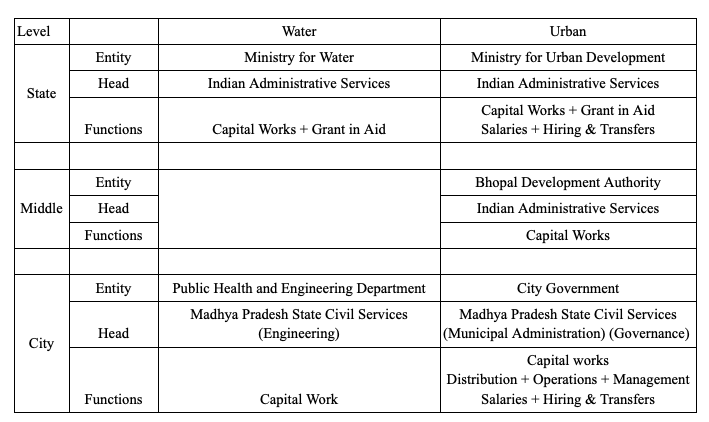
\includegraphics[width=1\textwidth]{images/Bwater.png} % Adjust the width as needed
    \caption{Bhopal's Administrative Water Delivery Chart. Source: Different Sources}
   
\end{figure}


Bhopal's successful water governance largely stemmed from its effective use of state-level bureaucrats recruited through the Madhya Pradesh State Civil Services (Provincial Services). These officers, primarily from Municipal and General Administration cadres, served in crucial positions like Assistant and Additional Commissioners, bridging the gap between elite Indian Administrative Service (IAS) officers and frontline staff. Unlike their IAS counterparts who viewed urban postings as temporary career steps, Provincial Service officers maintained longer tenures in city assignments.In this respect, these state-level bureaucrats closely resemble their counterparts in Lucknow, where similarly recruited officers oversee both the city’s water utility (the Lucknow Jal Sansthan) and its municipal administration (the Lucknow Municipal Corporation). This continuity enabled these bureaucrats to develop deep local expertise and institutional memory while working within established administrative frameworks, ultimately contributing to more effective urban governance. As one state bureaucrat explained succinctly:
\begin{quote} “We are here for the rest of our lives. This is our work, and if we do not do this, who will?”\footnote{Interview with an officer of the Madhya Pradesh State Civil Services (Municipal Administrative Services Cadre). Bhopal 2022)
} \end{quote}

This embedded position allowed these officers to navigate the vertical hierarchies of elite IAS officials above them and the horizontal complexities of city departments and frontline staff below. Far from achieving full autonomy, they still had to accommodate legitimate political pressures and community demands. Yet their relative permanence and localized knowledge created a form of partial insulation—the crux of conditional autonomy—allowing them to maintain technical standards, initiate reforms, and adapt strategies over time.

The institutional framework enabling such bureaucratic intermediation took concrete shape through substantial development funding: \$346 million drawn from an Asian Development Bank (ADB), JnNURM and Department for International Development (DFID) which lasted from 2006-2014.\footnote{These funds were channeled through the Madhya Pradesh Urban Services for the Poor (MPUSP) and Madhya Pradesh Urban Water Supply and Environmental Improvement in Madhya Pradesh Project (MPUSEI) initiative, which included two flagship programs: UDAY (a loan by ADB) focused on strengthening physical infrastructure, and UTHAN (untied grant by DFID) targeted institutional reforms, better revenue management, and enhanced administrative practices. This flow was supported by JnNURM a reform contingent grant from the Union Government.} This infusion of capital did not simply erect infrastructure; it also reshaped bureaucratic practices.  Unlike Lucknow—where project units operated at a remove from municipal structures—Bhopal integrated its Project Implementation Unit (PIU) directly into the Bhopal Municipal Corporation (BMC).\footnote{Interview with the City Team Leader from DFID (2006-2009) Zoom 2021 2022.} International agencies also did more than supply funds: they adapted their oversight mechanisms to work within, rather than bypass, state structures, creating a rare synthesis between international development expertise and local institutional realities. 

The PIU assembled about 30 full-time professionals, including both consultants and state bureaucrats, all required to maintain a constant presence in Bhopal.\footnote{See annexure for the organizational design of PMU, PIU} The consultants’ technical expertise, external affiliations, and alignment with global governance norms enhanced the PIU’s standing. Their sustained involvement and proximity conferred a form of prestige and recognition often associated with external validation—what some scholars characterize as “symbolic capital” \citep{bourdieu_forms_1986}. Meanwhile, state bureaucrats, with long-term commitments to regional administration, contributed local knowledge and institutional memory. Although senior leadership (consultant team leaders and elite IAS project heads) frequently rotated, a core group of consultants and state officials remained, fostering stable relationships, shared norms, and collaborative problem-solving that bridged external expertise and local realities.\footnote{A project manager at the state level, typically an IAS officer, was appointed specifically to work with this group for a two-year term.}

Three key developments illustrate how this incremental capacity-building advanced the city’s governance norms. First, the Project Implementation Unit (PIU) deliberately diversified skill sets beyond engineering, incorporating procurement specialists, public finance professionals, and urban governance experts.\footnote{Interview with the officers of the Madhya Pradesh State Civil Services who were part of the PIU. Bhopal 2021 2022 2023} This broadened perspective reframed urban challenges—from water delivery to waste management—not as siloed engineering problems but as multifaceted governance issues involving human resources, coordination, and institutional design. By embedding these varied competencies, the PIU internalized new problem-solving approaches and routine practices. 

Second, capacity-building targeted systemic weaknesses in human resource management. City-level hiring had traditionally been influenced by patronage, leaving technical roles in engineering, sanitation, auditing, and public health under-skilled and unevenly staffed. Recognizing that these issues were not unique to Bhopal but endemic across Madhya Pradesh’s urban sector, state-level bureaucrats leveraged their embedded position to initiate institutional reforms.\footnote{Interview with Devinder Chauhan, Madhya Pradesh State Administrative Services, Bhopal, 2022. This version was corroborated by Bruce Pollock and Jim Arthur, both of whom were DFID officers in Madhya Pradesh. Zoom 2022, 2023.
} One officer complained that District Magistrate (DM)-oriented IAS training “didn’t prepare them for cities":

\begin{quote}
    “Other cities [like Gwalior, Indore, Jabalpur, and Ujjain] faced similar issues. We raised these staffing concerns with the Commissioner, but they didn’t prioritize them. Urban is a very small part of a District; officers mostly deal with schemes for rural areas. Their field training as District Magistrates (DMs) didn’t prepare them for cities.  \textit{Woh municipal ko samjah hi nahin sakte} (They cannot understand cities).”\footnote{Interview with an officer of the Madhya Pradesh State Civil Services (Municipal Administrative Services Cadre).
Bhopal 2022}
\end{quote}

Another added 

 \begin{quote}
“These engineers, tax inspectors would be our problem in the long term. We have to face them [for the entire duration of their career], not those in the \textit{Sachivalaya} (Secretariat).”\footnote{Interview with an officer of the Madhya Pradesh State Civil Services (Municipal Administrative Services Cadre).
Bhopal 2022}

 \end{quote}

 These reflections underscore a power dynamic and professional identity distinct from the IAS-dominated paradigm. The state cadre officers, more deeply embedded in urban contexts, leveraged their position to introduce reforms that aligned long-term city interests with institutional capabilities. By pushing beyond conventional hiring patterns, these officers created conditions where stable, competency-driven staffing could emerge as the norm. Collaborative exercises motivated by these state bureaucrats culminated in the creation of a Standard Departmental Structure, comprising 10 departments and 110 designations, alongside the establishment of five new municipal cadres—Accounts, Revenue, Engineering, Sanitation, and Executive services—and a revision of Service Rules to institutionalize these changes.\footnote{Oxford Policy Management. (2012). \textit{Project completion review: Madhya Pradesh Urban Services for the Poor (MPUSP) Project}. Available at: \nolinkurl{https://iati.fcdo.gov.uk/iati_documents/3780261.odt}} This internal cadre reform geared towards the cities, was not simply a technical adjustment; it represented the codification of new norms into formal structures. An independent end of project evaluation  acknowledged: “[It] appreciates the above interventions that had to overcome considerable on-ground challenges.”\footnote{ibid., page 9}

A third issue—how to sustainably ramp up capacities over time—centered on core public management tasks. In the 2000s, BMC faced challenges common to Indian cities: procurement, tender preparation, quality control, and complex Management Information Systems (MIS) implementation. The DFID grant provided specialists in administration, e-governance, communications, finance, engineering, social development, GIS, and energy.\footnote {Proposal for Financial Assistance Under Madhya Pradesh Urban Services for the Poor (MPUSP) Programme, Department for International Development (DFID), January 2007, Bhopal.}
However, the impetus for these changes did not come solely from elite IAS officers; the groundwork was laid by the state bureaucrats who engaged directly with frontline bureaucrats—tax assessors, computer operators, engineers, and others—to institutionalize these changes. Over time, state cadre officers developed technical expertise in tendering, procurement, and advanced tools like GIS and MIS. Large-scale training initiatives—12,000 city government staff trained across six cities, including Bhopal—further strengthened these emerging competencies.\footnote{Oxford Policy Management. (2012). \textit{Project completion review: Madhya Pradesh Urban Services for the Poor (MPUSP) Project}. Available at: \nolinkurl{https://iati.fcdo.gov.uk/iati_documents/3780261.odt}} From a theoretical standpoint, these capacity-building efforts represent a form of social learning and collective adaptation. As bureaucrats gained new skills and witnessed the benefits of improved procedures, these practices became internalized as standard operating procedures. This gradual normalization of improved management and technology adoption created norms which spread via professional networks, path dependence, and the pursuit of organizational legitimacy.

The property tax reforms exemplify how these reforms produced tangible, if partial, results. As in Lucknow, external financing conditions required municipal revenue improvements. However, raising water tariffs proved politically contentious, as political resistance at the city and state levels , similar to Lucknow stymied any moves toward metering or pricing increases.\citep{sen_issues_2022} A DFID team leader observed:

\begin{quote}
    "This was not just Bhopal. Getting politicians in India to increase tariffs is a problem. We tried to convince the bureaucrats, actually—that, I think, was the key to our work. Our strategy was to talk to the bureaucrats, and they would then talk to the politicians."\footnote{Interview with Dr Bruce Pollock, Project Manager Kathandu Nepal 2022 Zoom 2024}
\end{quote}

DFID was encouraged by the state cadre officers to focus on expanding the property tax base instead of pushing politically sensitive water tariff hikes. With only 46\% of properties taxed, this represented a substantial revenue opportunity.\footnote{\textit{Budget document, Lucknow Municipal Corporation}, 2005–2014.} The state officers in their field experience as well as inputs from the revenue officers noted that the base was low and if increased to 90\% of properties - a move that would substantially increase municipal revenue without requiring politically sensitive rate hikes. This approach sidestepped direct political opposition to metering or price increases, aligning bureaucratic goals with political interests more smoothly.  

Below is a revised version that aims for greater clarity and coherence:

The expansion of Bhopal's property tax base was guided by a systematic, state bureaucrat–led strategy. Officers were first trained in property evaluation techniques and began by surveying newer areas before moving on to established neighborhoods. This phased approach was bolstered by technical innovations such as GIS mapping and automated tax calculation tools, which together produced an integrated property database linked to cadastral records and revenue maps \citep{awasthi_property_2020}. A key milestone in this process was the introduction of a centralized Management Information System (MIS)—making Bhopal the second Indian city, after Mumbai, to implement one.\footnote{The implementation of the MIS is discussed in detail in the chapter on Trash.}

To support these changes, state bureaucrats navigated political resistance to digital modernization and expanded on-the-ground capacity by increasing the number of tax assessors from 22 to 148. They institutionalized regular monitoring through monthly meetings on door-to-door surveys and introduced unique household property IDs.\footnote{Oxford Policy Management. (2012). Project completion review: Madhya Pradesh Urban Services for the Poor (MPUSP) Project. Available at: \url{https://iati.fcdo.gov.uk/iati_documents/3780261.odt}} Attention to both technical and administrative details underpinned the reform’s success. State bureaucrats regularly updated tax registers, established grievance redressal mechanisms within municipal offices, and managed political demands for tax amnesties and exemptions. In doing so, they maintained the integrity of the system while accommodating legitimate concerns.


In Bhopal, while property tax reforms significantly bolstered revenue administration—with collections rising from \$3.73 million in 2006–07 to \$9 million in 2011–12—dependence on state and union grants persisted.\footnote{Proposal for Financial Assistance Under Madhya Pradesh Urban Services for the Poor (MPUSP) Programme, Department for International Development (DFID), January 2007, Bhopal.} Meanwhile, revenue from water remained negligible, as only 3\% of households had meters in 2022, indicating the political reluctance to tackle more contentious reforms like raising water tariffs. This partial success illustrates a familiar dynamic: technical and administrative reforms can tackle immediate, manageable issues but rarely overcome entrenched political and structural barriers. From a theoretical standpoint, this outcome aligns with the notion that state-level bureaucrats often succeed with “low-hanging” administrative fixes—such as broadening the property tax base—but struggle to secure political support for more challenging measures. The reluctance to confront the politically sensitive issue of water charges underscores how technical progress can coexist with underlying governance dilemmas. Yet, by focusing on what was politically feasible—enhancing skill sets, standardizing departments, and improving procurement and MIS systems—state cadre officers and their allies created a more resilient administrative environment. Although these adjustments did not fundamentally alter the political economy of urban service delivery, they established a crucial foundation for addressing more complex issues of political-business relations and community engagement, topics explored in the following sections. In this sense, the Bhopal case illustrates that bureaucratic intermediation, while not transformative in itself, can still produce meaningful gains amid persistent political constraints.


\subsection{Managing Political-Business Relations: The Art of Bureaucratic Intermediation}

The previous section outlined how Bhopal’s state-level bureaucrats gradually built institutional capacity and internalized new governance norms, reinforcing the partial insulation central to conditional autonomy. Another, more intricate challenge emerged as significant development funding—approximately \$346 million from various agencies—flowed into the city. Now, beyond just ensuring technical proficiency and incremental reforms, bureaucrats had to manage the political economy of large-scale infrastructure projects. This elevated the stakes considerably: politicians viewed these funds as potential patronage opportunities, and local contractors—despite their experience in small-scale work—struggled with advanced technical standards demanded by international funders. As these massive projects got underway, rather than operating under full insulation or succumbing to pure instrumentalization, these officials found themselves navigating a contested space where political pressures and market forces converged. They needed to uphold minimum quality standards and maintain project coherence, even as political actors pushed for favoritism and contractors lobbied for easier conditions. Merely applying formal procurement guidelines or technical manuals was insufficient. The situation called for informal negotiation, persuasion, and adaptive strategies.

The unprecedented scale of development funding created new political–business dynamics.  Local contractors, skilled at small-scale municipal works, suddenly faced FIDIC-based contracts \footnote{FIDIC (Fédération Internationale Des Ingénieurs-Conseils) contracts are standardized construction contracts developed by the International Federation of Consulting Engineers. These contracts set global standards for complex infrastructure projects, including detailed specifications for risk allocation, quality control, and dispute resolution. While standard in international development projects, they marked a significant departure from traditional municipal contracting practices in Indian cities.}, stringent quality thresholds, and global best practices. This mismatch created instability: opaque procurement rules, lowest-bidder selection criteria, and a dearth of familiarity with ADB procedures produced confusion and risk premiums.\footnote{Proceedings from the MP Urban (ADB) Project at the R.C.V.P. Noronha Academy of Administration and Management Bhopal on "Procurement under MP Urban (ADB) Project".} Existing arrangements—where internal settlements and “lowest bidder wins” often led to substandard work.\footnote{Interview with Dr Bruce Pollock, Project Manager (2006-2009) Kathandu Nepal 2022 Zoom 2024} Without actors capable of bridging information gaps, interpreting technical requirements, and mediating disputes, implementation would have stalled.

Here, state bureaucrats emerged as essential mediators. While consultants ensured formal compliance, they alone could not unravel the complex interplay of political patronage, contractor ambitions, and administrative constraints. Politicians, anticipating new patronage channels, pressured to direct contracts to favored firms. Some contractors with checkered pasts but strong political links sought re-entry into bidding.\footnote{Chouhan, S. S. (n.d.). Transforming Madhya Pradesh. Skoch Group. Retrieved from https://books.skoch.in/shop/books/transforming-madhya-pradesh-shivraj-singh-chouhan/} Elite IAS officers, steeped in formal roles and wary of compromising professional neutrality, hesitated to intervene directly. State-level officers, by contrast, leveraged their unique position—characterized by long-term urban postings and deep local networks—to bridge these divides. They recognized that formal procurement rates often failed to reflect market realities, creating perverse incentives for corruption and compromised quality. Their response was multi-tiered: public consultative meetings addressed formal bidding processes,\footnote{Meeting records show that contractors themselves raised concerns about corruption among city engineers. Politicians, meanwhile, pointed to bureaucratic intransigence and favoritism - a circular blame game ensued. } while smaller "vision alignment" sessions provided space for stakeholders to air grievances and negotiate workable solutions. Through these iterative negotiations, state bureaucrats developed practical innovations. They restructured large projects into smaller "packages" accessible to local contractors while maintaining quality standards. They worked with consultants to clarify technical requirements and adjusted tender specifications to reflect realistic costs. This approach did not eliminate informal practices but channeled them into more transparent, manageable arrangements. The result was a pragmatic framework that balanced political imperatives with administrative necessities.

Bhopal’s then-Mayor, Sunil Sood, candidly encapsulated these political realities.

\begin{quote}
``\textit{Thekedar} (Contractors) are a vital part of the process and an essential component of the world we work in. I am in power now, tomorrow I am in the opposition. If I will not accommodate their interests [contractors linked with opposition city leaders], why will they accommodate mine?"\footnote{Interview with Sunil Sood, Congress led Mayor of Bhopal City Government (2004-2009), Leader of Oppostion (2009-2012) Leader of Bhopal City Council (2000-2004), City Councillor (1995-2009). Bhopal 2021, 2022, 2023) 
}
\end{quote}

This statement underscores the political realities that formal institutional designs rarely capture. Similarly, the then Project Director from the elite IAS 
 cadre, Manish Singh, acknowledged the complexity:

\begin{quote}
``You can understand the implications of getting these contractors in the office. Negotiating is not my job, its the politicians. But  we as bureaucrats also have to get involved... I did ask my deputies to look into this—they knew the landscape better."\footnote{Interview with Manish Singh, Project Director - Madhya Pradesh Urban Services Improvement Program}
\end{quote}

These comments reveal a crucial distinction: while elite IAS administrators maintained formal distance, state bureaucrats engaged directly in day-to-day negotiations. Their long-term presence in the system provided them with institutional memory and deep local networks. Acting as boundary spanners \citep{tushman_boundary_1981}, they bridged the gap between politicians, contractors, and consultants. Unlike IAS officers constrained by formal rules and expectations of political neutrality, these state bureaucrats could work through informal channels, leveraging their relationships to secure resources and build consensus among stakeholders.



\begin{table}[ht]
\centering
\begin{tabular}{l l l l}
\toprule
\textbf{State} & \textbf{Capital Works} & \textbf{Operations \& Management} & \textbf{Revenue Functions} \\
\midrule
Madhya Pradesh    & State \& City Government        & City Government                   & City Government \\
Uttar Pradesh     & State \& City Government        & Parastatal \& City Government     & Parastatal \& City Government \\
Andhra Pradesh    & State                           & City Government                   & City Government \\
Bihar             & State                           & State                             & City Government \\
Chhattisgarh      & State                           & State                             & City Government \\
Gujarat           & State \& City Government        & City Government                   & City Government \\
Himachal Pradesh  & State                           & State                             & City Government \\
Karnataka         & State \& City Government        & City Government                   & City Government \\
Kerala            & State                           & State                             & State \\
Maharashtra       & State \& City Government        & City Government                   & City Government \\
Orissa            & State                           & State                             & State \\
Rajasthan         & State                           & State                             & State \\
\bottomrule
\end{tabular}
\caption{Overview of responsibilities in various Indian states.}
\label{tab:state-functions}
\end{table}





A pivotal episode narrated by the Mayor captures this delicate equilibrium. When contractors claimed rising material costs made current rates untenable, the Mayor convened a meeting of all stakeholders—engineering staff from the Public Health and Engineering Department (PHED), contractors, councilors—and tasked a state bureaucrat leading the Bhopal PIU and his team to mediate. As the Mayor recalled:

\begin{quote}
    “During my tenure, all this JnNUURM money came in. Work continued for eight years and the prices of pipes and earthwork rose, prompting the contractors to say they couldn’t continue at the current rates. Naturally, we couldn’t just approve higher rates without proper scrutiny. So I asked Mayan [State bureaucrat and Urban Governance Officer in the PIU] to bring his team. Everyone involved—engineering staff and contractors, councilors —and had them sit down together. I told them, ‘Look, we’re willing to consider what’s reasonable, but you can’t simply top-up on another 5-6\%. Then I asked directly, ‘How much commission is being paid here?’
The room went silent. I pointed out that the people who pay commissions and those who receive them are in the room, so there was no point hiding it. Eventually, they [contractors] admitted that the commission [to engineers of the PHED] of the amounted to around 12-14\%. I said, ‘Cut it down. If you’re giving 12\%, bring it down to about 5\%.  Mayank asked the chief engineer if this was an acceptable arrangement. He [Mayank] told them when there were no big projects, nobody made much. This is a 500 crores (about \$100 million) project, if this is delivered, more will come.’”\footnote{Interview with Sunil Sood, Congress led Mayor of Bhopal City Government (2004-2009), Leader of Oppostion (2009-2012) Leader of Bhopal City Council (2000-2004), City Councillor (1995-2009). Bhopal 2021, 2022, 2023) 
}
\end{quote}

These interactions were themselves a form of political signaling, where contractors and politicians used the meeting as a platform to communicate their demands and expectations. When quizzed about this corruption in general and this particular meeting in particular, the bureaucrat suggested how the contractors had to be involved in the way that the politicians wished: 

\begin{quote}
    “There are two kinds of pressure that politicians put on us: one is positive pressure, where public work needs to be done and they protest if it doesn’t happen accordingly. The other is negative pressure, where politicians pressure us to give their people contracts or withhold contractors’ payments. These meetings are part of that negative pressure—the contractors and politicians talk, and they want us to know what they want. You have to work in this framework, otherwise nothing would have happened.” \footnote{Interview with Mayank, Madhya Pradesh Administrative Services (Governance Cadre) Urban Governance Officer PIU Bhopal 2022
}
\end{quote}

Such negotiations reflect not a moral endorsement of corruption but a strategic containment approach consistent with the logic of conditional autonomy. Rather than an idealized “co-production” process free from rent-seeking, what occurred was a negotiated settlement where everyone aligned on a “doable” compromise. The state-level bureaucrats accepted certain informal practices as given, yet shaped them to protect minimum quality and efficiency standards. They leveraged their informal networks and standing as long-term urban administrators to reduce exaggerated commissions, insist on minimal technical thresholds, and subdivide contracts to lower barriers for local contractors. This recalibration prevented project collapse and ensured forward momentum—“getting things done” amid complexity and entrenched interests.

\vspace{12mm}

Consultant involved on the behalf of DFID elaborated:

\begin{quote}``We know there would be corruption, but what we cared about was the end outcome... These bureaucrats faced similar challenges in other cities as well, so we provided them with broad contours of the project, but they had to do the coordination and we tried our best to accommodate.”\footnote{Interview with Richard Slater, Governance Advisor 2009-2012 PIU. Tripline Consultancies} \end{quote}

This statement emphasizes that state-level bureaucrats were not merely implementing predetermined policies; they were actively shaping the project’s trajectory through negotiated intermediation. This instance exemplifies conditional autonomy in moments when elite IAS officers granted minor freedoms. Although not fully insulated from political pressures nor entirely captured by them, these bureaucrats adapted and leveraged informal norms—such as the “vision meetings” mentioned here—to achieve workable compromises. This scenario aligns with theories suggesting that in low-capacity environments, certain informal arrangements, while normatively undesirable, can serve as “lubricants” facilitating the execution of large-scale infrastructure projects.


Bhopal’s experience thus reveals that “getting things done” in complex institutional contexts often involves balancing political demands, contractor interests, and technical standards. State-level bureaucrats, with their dual role as “intermediaries within and outside the state,” managed to navigate these conflicting objectives without completely surrendering to either political patronage or technocratic rigidity. In effect, the state bureaucrats’ approach deviates from idealized governance models but still advances some developmental goals. By containing and structuring informality—reducing exaggerated commissions, insisting on minimal quality thresholds, subdividing contracts to lower barriers to entry—they constructed a more manageable political-business environment. These partial controls and incremental adjustments reinforced a set of emerging norms and practices consistent with conditional autonomy. Thus, rather than weakening the case for institutional reform, these actions underscore the complexity of governance challenges and the nuanced role that officials play in forging workable solutions under less-than-ideal conditions.

Having illustrated how state bureaucrats moderated political-business relations, I now move to the final dimension of Bhopal’s conditional autonomy: legitimizing community participation and addressing the persistent gap between infrastructure creation and sustainable, equitable service delivery

\subsection{Beyond Infrastructure: The Limits of Conditional Autonomy in Service Delivery}

Having seen how state-level bureaucrats in Bhopal moderated political-business relations to push large-scale projects forward, I now consider another aspect: ensuring that the expansions in infrastructure translate into sustainable, equitable service delivery. Thus far, I have identified these state officers as pivotal intermediaries—operating both within and outside the state—to accommodate political pressures and market imperatives without collapsing into pure patronage or rigid technocracy. Yet, their engagement with slum communities reveals both the promise and the limitations of this approach. While bureaucratic intermediation improved access and legitimacy, it struggled to deliver consistently high-quality services, illustrating what the I call “precarious universalism.”

Delivering water to Bhopal’s slums laid bare the complexity of local political and bureaucratic economies. Politicians, who wielded influence over pipeline extensions, tanker allocations, and borewell installations, often used these resources selectively, reinforcing patterns of patronage.\citep{auerbach_neighborhood_2017} In some instances, certain marginalized groups—migrants, religious minorities, Dalits, and Tribals—found themselves systematically deprioritized. Meanwhile, frontline engineering staff and field-level workers extracted petty rents by controlling pump schedules or influencing maintenance decisions.  Although DFID’s grant required prioritizing slums in public goods delivery, my interviews and field observations suggest that the complexity of local political economies and bureaucratic hierarchies demanded more than a top-down reform agenda.  Instead, state-level bureaucrats had to step in as credible intermediaries who could legitimate community-driven solutions while maintaining at least minimal adherence to technical and administrative standards.

DFID’s emphasis on slum improvement offered an opening to challenge these patterns. With Bhopal ranking 13th among India’s 132 cities in terms of slum population, the scale of the task was immense. Baseline surveys reported only 30\% piped water coverage in slums, with most residents traveling significant distances for basic needs. In principle, DFID’s protocols called for partnering with Non Governmental Organizations (NGOs) to foster community participation (Figure 1.7).\citep{kutter_demystifying_2014} Yet as one Mayor derisively put it,—``Woh toh paisa banne wale log hai. Na idhar ki baat karte hai no udhar ki" (“They’re just there to make money; they neither speak for here nor there”) \footnote{Interview with Krishna Gaur, Mayor of Bhopal (2009-2014), Bhopal 2021, 2023}— civil society organizations  lacked both entrenched urban poverty expertise and the political trust necessary to challenge established bureaucratic and political interests. Building legitimacy and meaningful engagement required a different catalyst.

\begin{figure}[H] % Use [H] to force the image to appear exactly where you place it
    \centering
    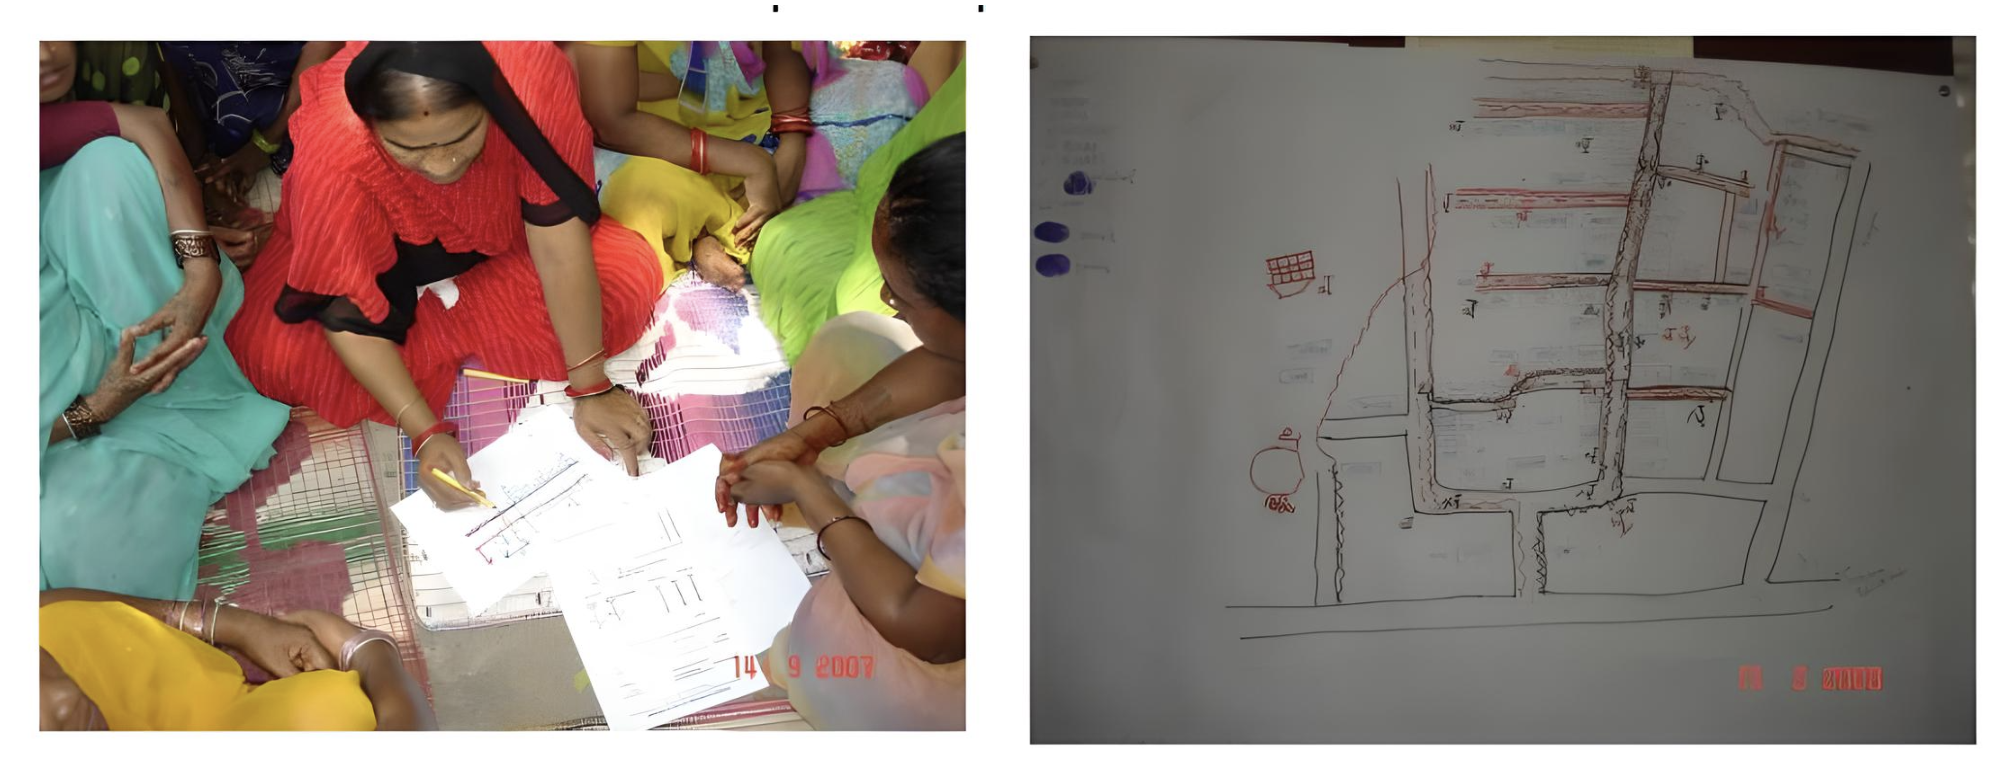
\includegraphics[width=1\textwidth]{images/Screenshot 2024-12-14 at 17.16.40.png} % Adjust the width as needed
    \caption{Left: Slum Management Committees working with civil society members under the DFID project. Right: Neighborhood Map for audit. Source: Provided by NGO SAMARTHAN. Bhopal 2022}
   
\end{figure}



Here again, state-level bureaucrats performed a critical bridging function. They worked with NGOs—sometimes reluctant partners—and formed community committees to oversee contractor performance.\citep{kumar_barriers_2016} Crucially, DFID’s requirement for public hearings before releasing payments to contractors granted these committees a formal oversight tool. While frontline staff and contractors might collude to justify incomplete work, committees armed with official sanction and supported by recognized bureaucrats could push back. As one NGO representative noted:
\begin{quote} “When these state bureaucrats would come visit, they also made sure other department officers came—water works, urban development, revenue, and municipal corporations. Our presence was legitimized if the officer was there; otherwise, we were not that important.”\footnote{Interview with members of AARAMB, Bhopal based civil sociey organization. Bhopal 2022, Zoom 2024} \end{quote}


Pushed by DFID on the top and the civil society organization in the bottom, state-level bureaucrats lent their institutional authority—and their embedded networks in the city administration—to turn community committees from nominal watchdogs into actors with real leverage. They thus moved beyond mere facilitation to active legitimization of community-driven solutions. In slums like Bagmugaliya,\footnote{established in 1983Despite having 148 households and a population of 740, this slum had no regular water source and relied entirely on tanker supply. }  residents pooled resources to create localized piped networks or install pumps, despite such measures being technically “illegal” or at least noncompliant with municipal regulations.\citep{noauthor_poverty_2006} Similar grassroots solutions emerged elsewhere—one community financed a pump to serve uphill residences; another built a common septic tank. Municipal guidelines deemed such arrangements improper due to issues like inadequate pipe depth or lack of structural integrity. Post-2014 regulatory shifts learned and even allowed some previously informal solutions to be integrated into municipal systems.


By reframing these improvised infrastructures as necessary stopgaps toward last-mile connectivity, bureaucrats convinced frontline staff and even some IAS superiors to tolerate these arrangements. Involving elected officials ensured political cover, while consulting technical experts and setting minimal performance standards prevented egregious risks. This delicate balancing act exemplifies conditional autonomy in action: bureaucrats operating in a gray zone, between strict enforcement of regulations and total political acquiescence, crafting pragmatic compromises that advanced coverage—if not impeccable compliance.\footnote{ As one civil society organization observed, "the authorization for the same has to come from the elected officials... and through negotiations with the frontline and upper-tier bureaucrats." The bureaucrats' ability to convert potentially contentious informal arrangements into accepted practice, while maintaining program objectives and getting street-level bureaucrats and politicians on board, was crucial for success.}
 

Yet these accomplishments came with clear constraints. While pipes and pumps proliferated, consistent water pressure and reliability lagged behind. Field research and citizen surveys revealed a stark contrast: although near-universal access (93\% in shacks, 97\% in slums) was achieved, about 70\% of shack residents and 36\% of slum households received water for only one hour per day (Table 1.6 and Figure 1.8). This illustrates “precarious universalism”: a condition where coverage becomes widespread, but remains unstable and uneven. The system could easily revert to earlier dysfunction once external oversight or donor involvement subsided.


\begin{table}[ht]
\centering
\renewcommand{\arraystretch}{1.3} % Adjust row height
\setlength{\tabcolsep}{5pt} % Adjust column spacing
\begin{tabular}{|p{3cm}|p{3cm}|p{3cm}|p{3cm}|p{3cm}|}
\hline
\textbf{City} & \textbf{Housing Type} & \textbf{Tap (Piped)} (\%) & \textbf{Borewell + Hand Pump} (\%) & \textbf{Other Sources} (\%) \\ \hline
Bhopal & Shack & 93 & 1 & 6 \\ \cline{2-5}
       & Slum  & 97 & 2 & 1 \\ \hline
Lucknow & Shack & 48 & 37 & 15 \\ \cline{2-5}
        & Slum  & 64 & 32 & 4 \\ \hline
\multicolumn{5}{l}{\textit{Source: Primary survey under the Brown - India Citizenship Project 2022}} \\ % Add source note
\end{tabular}

\caption{Source of Water by City and Housing Type (Shack and Slum Only)}
\label{tab:water_shack_slum}
\end{table}



\begin{figure}[H] % Use [H] to force the image to appear exactly where you place it
    \centering
    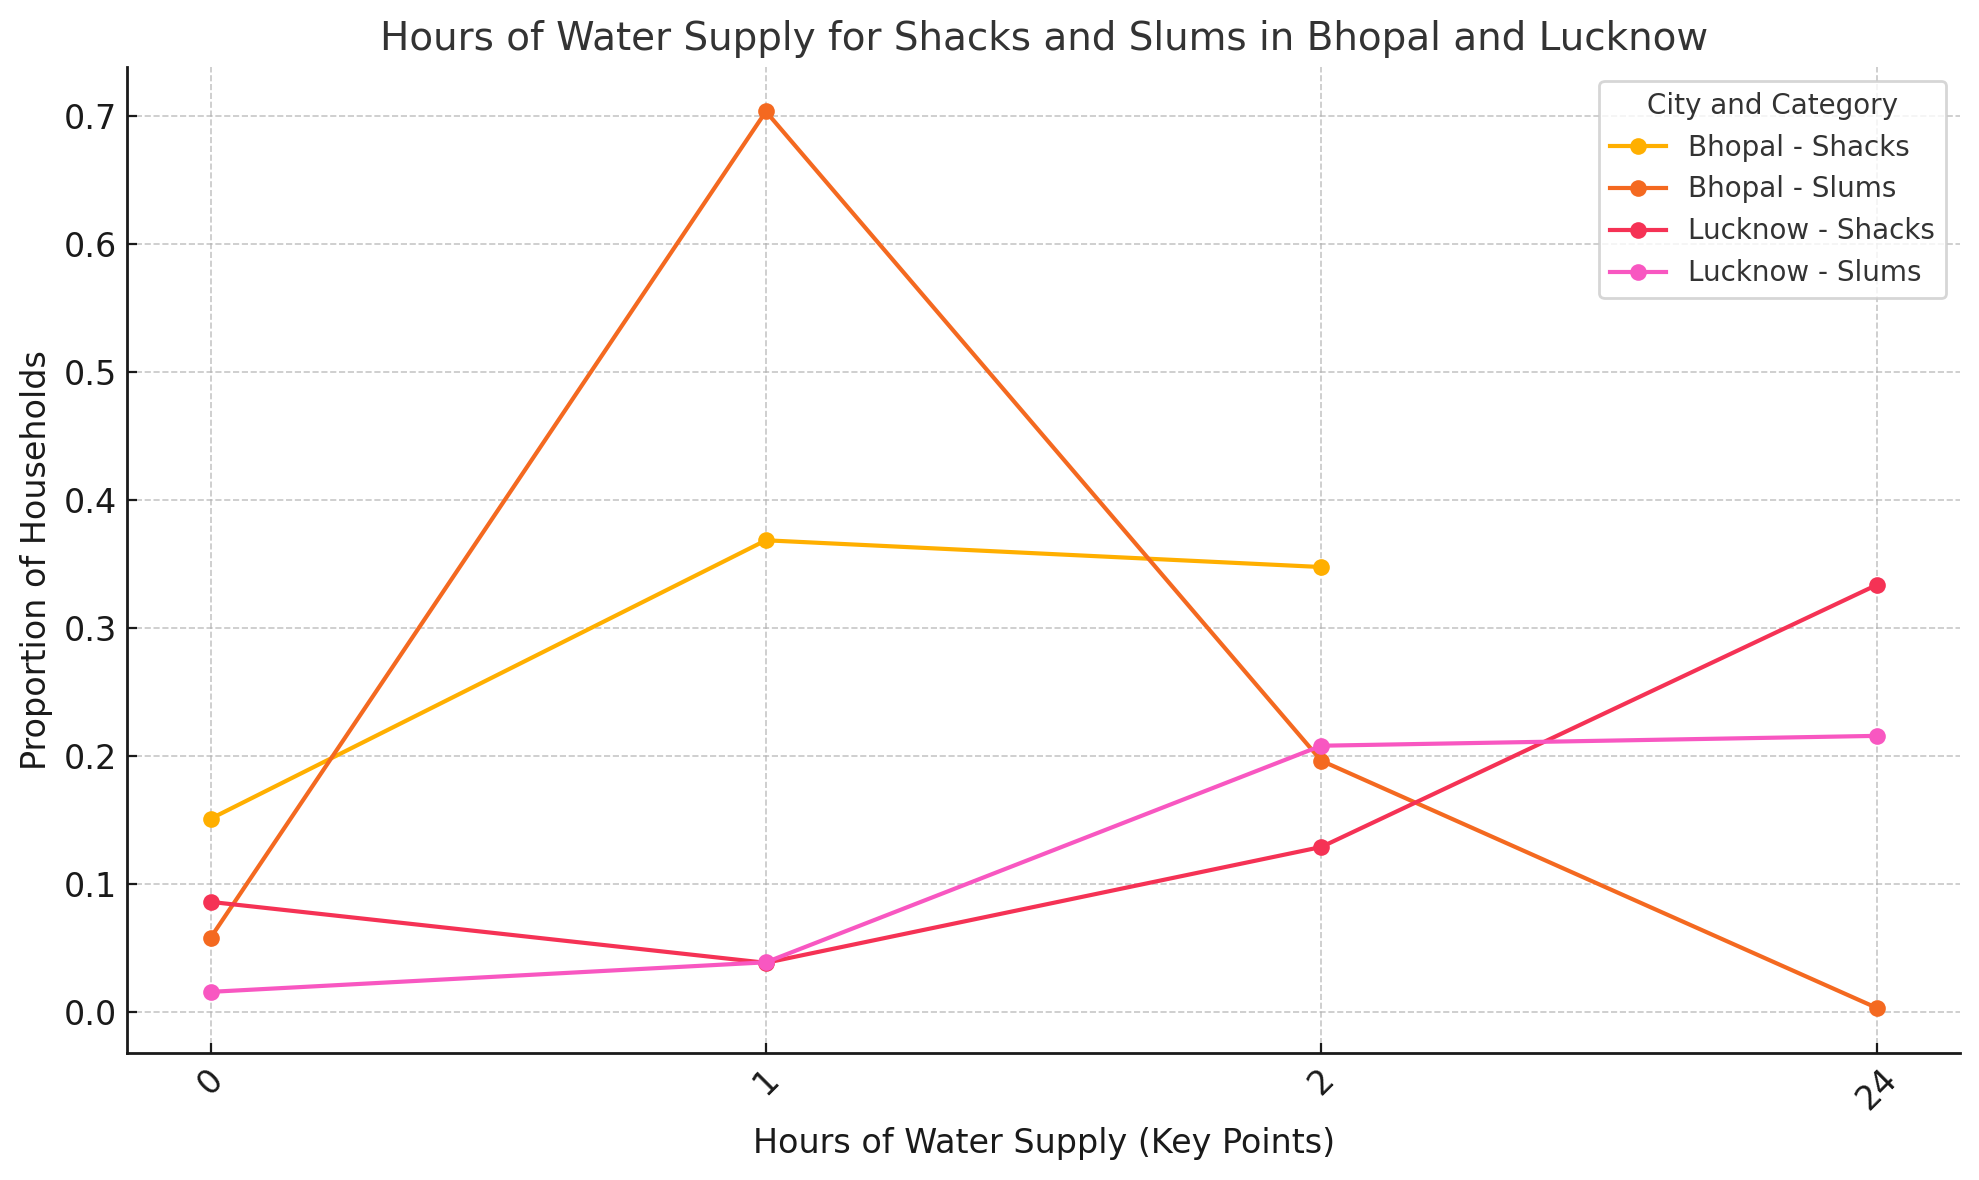
\includegraphics[width=1\textwidth]{images/water comparison-slum and shack.png} % Adjust the width as needed
    \caption{Hours of water suppply in the informal housing (slums and shacks) of Bhopal and Lucknow. Source: Primary survey under the Brown - India Citizenship Project 2022}
   
\end{figure}



While state-level bureaucrats could harness their unique position to overcome immediate implementation hurdles—navigating political pressures, adapting to local norms, and legitimizing community-driven solutions—they could not, on their own, sustain long-term improvements in service quality. Two main factors contributed to this constraint. First, bureaucratic incentives and donor metrics focused heavily on visible, quantifiable achievements—such as the number of new connections—rather than on long-term reliability or daily supply hours. Once external monitoring waned, maintenance and pressure management slipped, revealing the fragility of gains secured through negotiated compromises. Second, DFID’s intervention, though crucial in spurring community committees and slum focus, did not fundamentally alter the deeper political and institutional matrices governing service delivery. Entrenched patronage networks and frontline rent-seeking practices persisted. Without deeper transformations—empowering civil society beyond donor timelines, strengthening accountability mechanisms, and realigning political incentives—conditional autonomy could not evolve into a more genuinely programmatic or stable arrangement.

Bhopal’s experience in slum service delivery thus underscores both the strengths and inherent limits of bureaucratic intermediation under conditional autonomy. State-level bureaucrats could deftly navigate political-business conflicts, legitimize community participation, and secure widespread access, demonstrating the approach’s capacity for positive incremental change. Yet the enduring gap between infrastructural coverage and actual service quality, and the ease with which improvements could erode in the absence of sustained oversight, highlight that conditional autonomy is no panacea. Rather, it is a fragile equilibrium that can facilitate immediate progress but may struggle to deliver lasting institutional transformation.

In conclusion, while bureaucratic intermediation proved effective in surmounting immediate obstacles and achieving more inclusive coverage, ensuring consistent, high-quality service demands systemic changes that surpass the limited scope of these negotiated arrangements. Absent robust, long-term accountability structures, strong civil society engagement, and the reorientation of political incentives to value sustainability over short-term gains, precarious universalism will likely persist. Bhopal’s case, therefore, reinforces the idea that conditional autonomy—essential for navigating complexity and partial reform—is ultimately a stepping stone, not the final destination, in the pursuit of equitable and durable urban governance.

\subsubsection{Conclusion}
Bhopal’s trajectory illustrates that even in a context shaped by patronage politics, infrastructural complexity, and uneven bureaucratic capacity, state-level bureaucrats can forge a degree of conditional autonomy that yields meaningful gains. By embedding project management units within the municipal corporation, nurturing long-term professional cadres, and incrementally internalizing new norms, the city’s administration strengthened its ability to manage technical challenges, negotiate political-business relations, and incorporate community inputs—albeit within certain limits.

Throughout these sections, we have seen how this middle-ground arrangement deviated from both the ideal-type programmatic and the purely instrumental, patronage-driven model. Instead of achieving a fully insulated, programmatic environment, Bhopal’s state-level officials operated in a gray zone that tolerated some informal practices while imposing checks on rent-seeking. They adapted procurement rules, subdivided projects, engaged contractors in delicate negotiations, and legitimized community-driven solutions that bent, but did not break, formal standards. In doing so, they advanced public goods provision more effectively than their counterparts in Lucknow, while still falling short of stable, programmatic universalism.

Yet, Bhopal’s experience also underscores the fragile and partial nature of these accomplishments. Even with widespread coverage, service quality remained uneven, and the long-term sustainability of these gains was not assured. The persistent reliance on external funding, entrenched patronage networks, and weak civil society oversight left the system susceptible to reverting toward older patterns of fragmentation once donor involvement diminished or when political winds shifted. Conditional autonomy thus emerges not as a panacea, but as a pragmatic, adaptive framework that enables incremental improvements without guaranteeing lasting institutional transformation.

In sum, the Bhopal case offers a nuanced portrait of how embedded, mid-level bureaucrats—acting as intermediaries within and beyond the formal state structure—can navigate complexity, foster partial insulation, and negotiate workable compromises in infrastructural governance. These officials managed to deliver tangible benefits and more inclusive access, pushing the city beyond the low baseline of fragmentation. However, their achievements remained constrained by structural, political, and societal factors that conditional autonomy alone could not overcome. The lessons from Bhopal highlight both the possibilities and the inherent limitations of negotiated reforms in challenging urban contexts—insights that resonate beyond this single city and extend to the broader study of public goods provision under imperfect institutional conditions.

\section{Conclusion and Contribution}

This chapter has explored how bureaucratic intermediation—specifically, the capacity of state-level officials to navigate complex political, administrative, and technical landscapes—shapes the provision of urban water services.

In Lucknow, the absence of credible intermediaries, combined with a “Trishanku-like” institutional arrangement, left the city’s water governance in a state of chronic paralysis. Formal reforms and considerable external funding did not translate into coherent local authority or programmatic decision-making. Instead, collusive ties between political and bureaucratic actors, ambiguous mandates, and reluctance to devolve meaningful control to the city level resulted in persistent fragmentation. At every turn, attempts to rationalize tariffs, embed project units locally, or strengthen accountability mechanisms failed to overcome entrenched mistrust and top-down domination. Lacking the mediating role that state-level bureaucrats could have played, Lucknow’s water system remained trapped in institutional dysfunction, with local communities forced to rely on patchwork solutions that reinforced inequalities and precarious access.

Bhopal’s trajectory, by contrast, demonstrates that even within a patronage-ridden and capacity-constrained environment, state-level bureaucrats acting as intermediaries can carve out a workable space to improve coverage and quality. Here, incremental investments in technical capacity, procurement norms, and administrative routines were matched by selective accommodation of political and contractor interests. By embedding project units directly into city governance and nurturing a professional, though not fully insulated, cadre of officers, Bhopal’s officials balanced the demands of top-level political actors, the pressures of local businesses and contractors, and the need to incorporate community voices. Over time, these negotiated arrangements produced what we might call “precarious universalism”: a state of significantly broader coverage, partial restraint on rent-seeking, and improved responsiveness to marginalized communities. Yet Bhopal’s accomplishments, while real, remained inherently fragile. The conditional autonomy achieved did not fully dislodge the enduring structures of patronage and did not ensure consistently high-quality service. Once donor oversight diminished and political winds shifted, the sustainability of these gains remained uncertain.

Taken together, these cases underscore that the capacity to deliver complex public goods like piped water depends not simply on formal organizational designs, top-level administrative appointments, or significant funding infusions. Instead, it also hinges on how skilled bureaucrats mediate competing pressures: bringing some coherence to fragmented authority structures, containing rather than eliminating corruption and favoritism, and cultivating legitimacy through iterative engagement with political actors, contractors, and local communities. Conditional autonomy emerges as an analytical lens that explains how certain bureaucratic agents can modulate patronage-driven environments to produce more stable, if imperfect, service delivery outcomes. This does not imply that conditional autonomy is the end goal. Rather, it is a stepping stone that can shift service delivery away from the baseline of fragmentation and clientelism toward arrangements that are more inclusive, technically sound, and socially responsive, even if not yet fully universal or enduring.


I make four contributions:

First, the chapter refines theories of bureaucratic autonomy by introducing the idea of\textbf{ conditional autonomy}—a negotiated middle ground that emerges in settings where fully programmatic administration is not fully realized, yet governance is not wholly patronage-driven either. Classic theories often frame bureaucratic autonomy in idealized terms—either as a Weberian, rule-bound apparatus shielded from political intrusion or as a captured, instrumentally manipulated entity. The evidence from Bhopal’s water governance complicates this binary. Bureaucrats operate in a “gray zone,” maintaining enough insulation to preserve technical standards and long-term planning but never achieving full independence from political demands. Conditional autonomy thus expands our theoretical toolkit, showing that meaningful, if partial, reforms can occur even in environments where political pressures and informal practices persist. By highlighting how bureaucrats secure incremental improvements while navigating these constraints, this concept challenges rigid dichotomies and underscores the adaptive capacity of state actors in imperfect contexts.

Second, This dissertation’s focus on mid-level bureaucrats offers a fresh vantage point for understanding the machinery of governance. Rather than centering on top-tier elites who cycle rapidly through brief postings, or on frontline workers overwhelmed by daily operational demands, this approach zeroes in on the “missing middle”—the state-level officials who bridge these two extremes. By drawing insights from scholarship on embedded autonomy and institutional capacity (Evans \& Rauch 1999; Migdal 1988; Tsai 2007), it shows how these mid-level actors act as internal intermediaries. They translate high-level policies into practical solutions, foster horizontal coordination across fragmented agencies, and create vertical linkages that connect strategic objectives with street-level realities. Engaging directly with political actors, private enterprises, and community groups, they forge alliances and negotiate compromises that gradually stabilize service delivery systems. In the Indian context, long portrayed as “weak-strong” (Rudolph & Rudolph 1987), “failed developmental” (Herring 1999), “Sisyphean” (Kapur & Mukhopadhyay 2007), or “flailing” (Pritchett 2009), recognizing the role of these mid-level bureaucrats provides a nuanced understanding of how incremental yet meaningful progress unfolds. By highlighting their capacity to transform fragmented governance into coordinated, scalable, and more equitable arrangements, this research broadens our understanding of how to strengthen state capacities, not through grand top-down reforms alone, but by investing in the “missing middle.”


Third, While scholarship on urban governance increasingly recognizes incremental progress toward more equitable policy outcomes, existing accounts often highlight how gradual reforms and partial institutionalization create conditions for enduring improvements \citep{eduardo_politics_2021}. My comparative findings build on this perspective by emphasizing the critical role of mid-level bureaucratic intermediation. Rather than incremental gains emerging solely from stable political alliances, strong municipal oversight, or well-established professional norms, the experiences of Lucknow and Bhopal show that “conditional autonomy” among embedded bureaucrats enables them to maneuver within patronage-laden environments. Such strategic adaptation and selective insulation can translate formal reforms into tangible, if still fragile, advances in service delivery. This contributes to the broader literature by underscoring that incremental improvements are contingent achievements—shaped not only by external mandates and progressive agendas, but also by the capacity of bureaucrats to navigate complex political terrain and incrementally steer systems toward more inclusive, reliable public goods provision.

Lastly: Methodologically, this chapter in particular, but the dissertation in general takes an important step toward advancing scholarly understanding of bureaucratic governance by moving beyond three common limitations in existing research: the overreliance on static, cross-sectional analyses; the narrow focus on principal–agent frameworks or top-down developmental state models; and the insufficient attention to how formal and informal practices intersect at the frontline.\citep{pepinsky_bureaucracy_2017} Instead of limiting attention to a single moment of reform or a particular institutional arrangement, this research traces bureaucratic changes and adaptations over time. By examining how state-level bureaucrats, municipal authorities, and frontline actors respond to shifting political priorities, evolving donor agendas, and infrastructural investments across extended periods, it becomes possible to pinpoint not only what triggers episodes of fragmentation or cooperation but also how incremental adjustments accumulate into more durable patterns of institutional capacity or persistent deadlock.

Equally important, the dissertation employs a mixed-methods design that integrates large-scale administrative datasets, field interviews, and ethnographic insights. Rather than relying solely on principal–agent models or treating complex interventions as if they were implemented in top-down isolation, this approach reveals the subtle interplay between formal incentive structures and the informal norms that shape frontline discretion. Through systematic quantitative analysis complemented by qualitative richness, the study captures not only measurable changes—such as revenue collection or staff deployment patterns—but also the interpersonal negotiations, tacit understandings, and professional identities that drive real-world policy implementation. This holistic, empirically grounded perspective illuminates why some bureaucracies inch toward more equitable, reliable service delivery even amid patronage and fragmentation, while others remain trapped in cycles of institutional paralysis and collusive arrangements.


\section{Annexure}

\subsection{Organogram of the Project Management Unit and the Project Impementation, Project UDAY}

\begin{figure}[H] % Use [H] to force the image to appear exactly where you place it
    \centering
    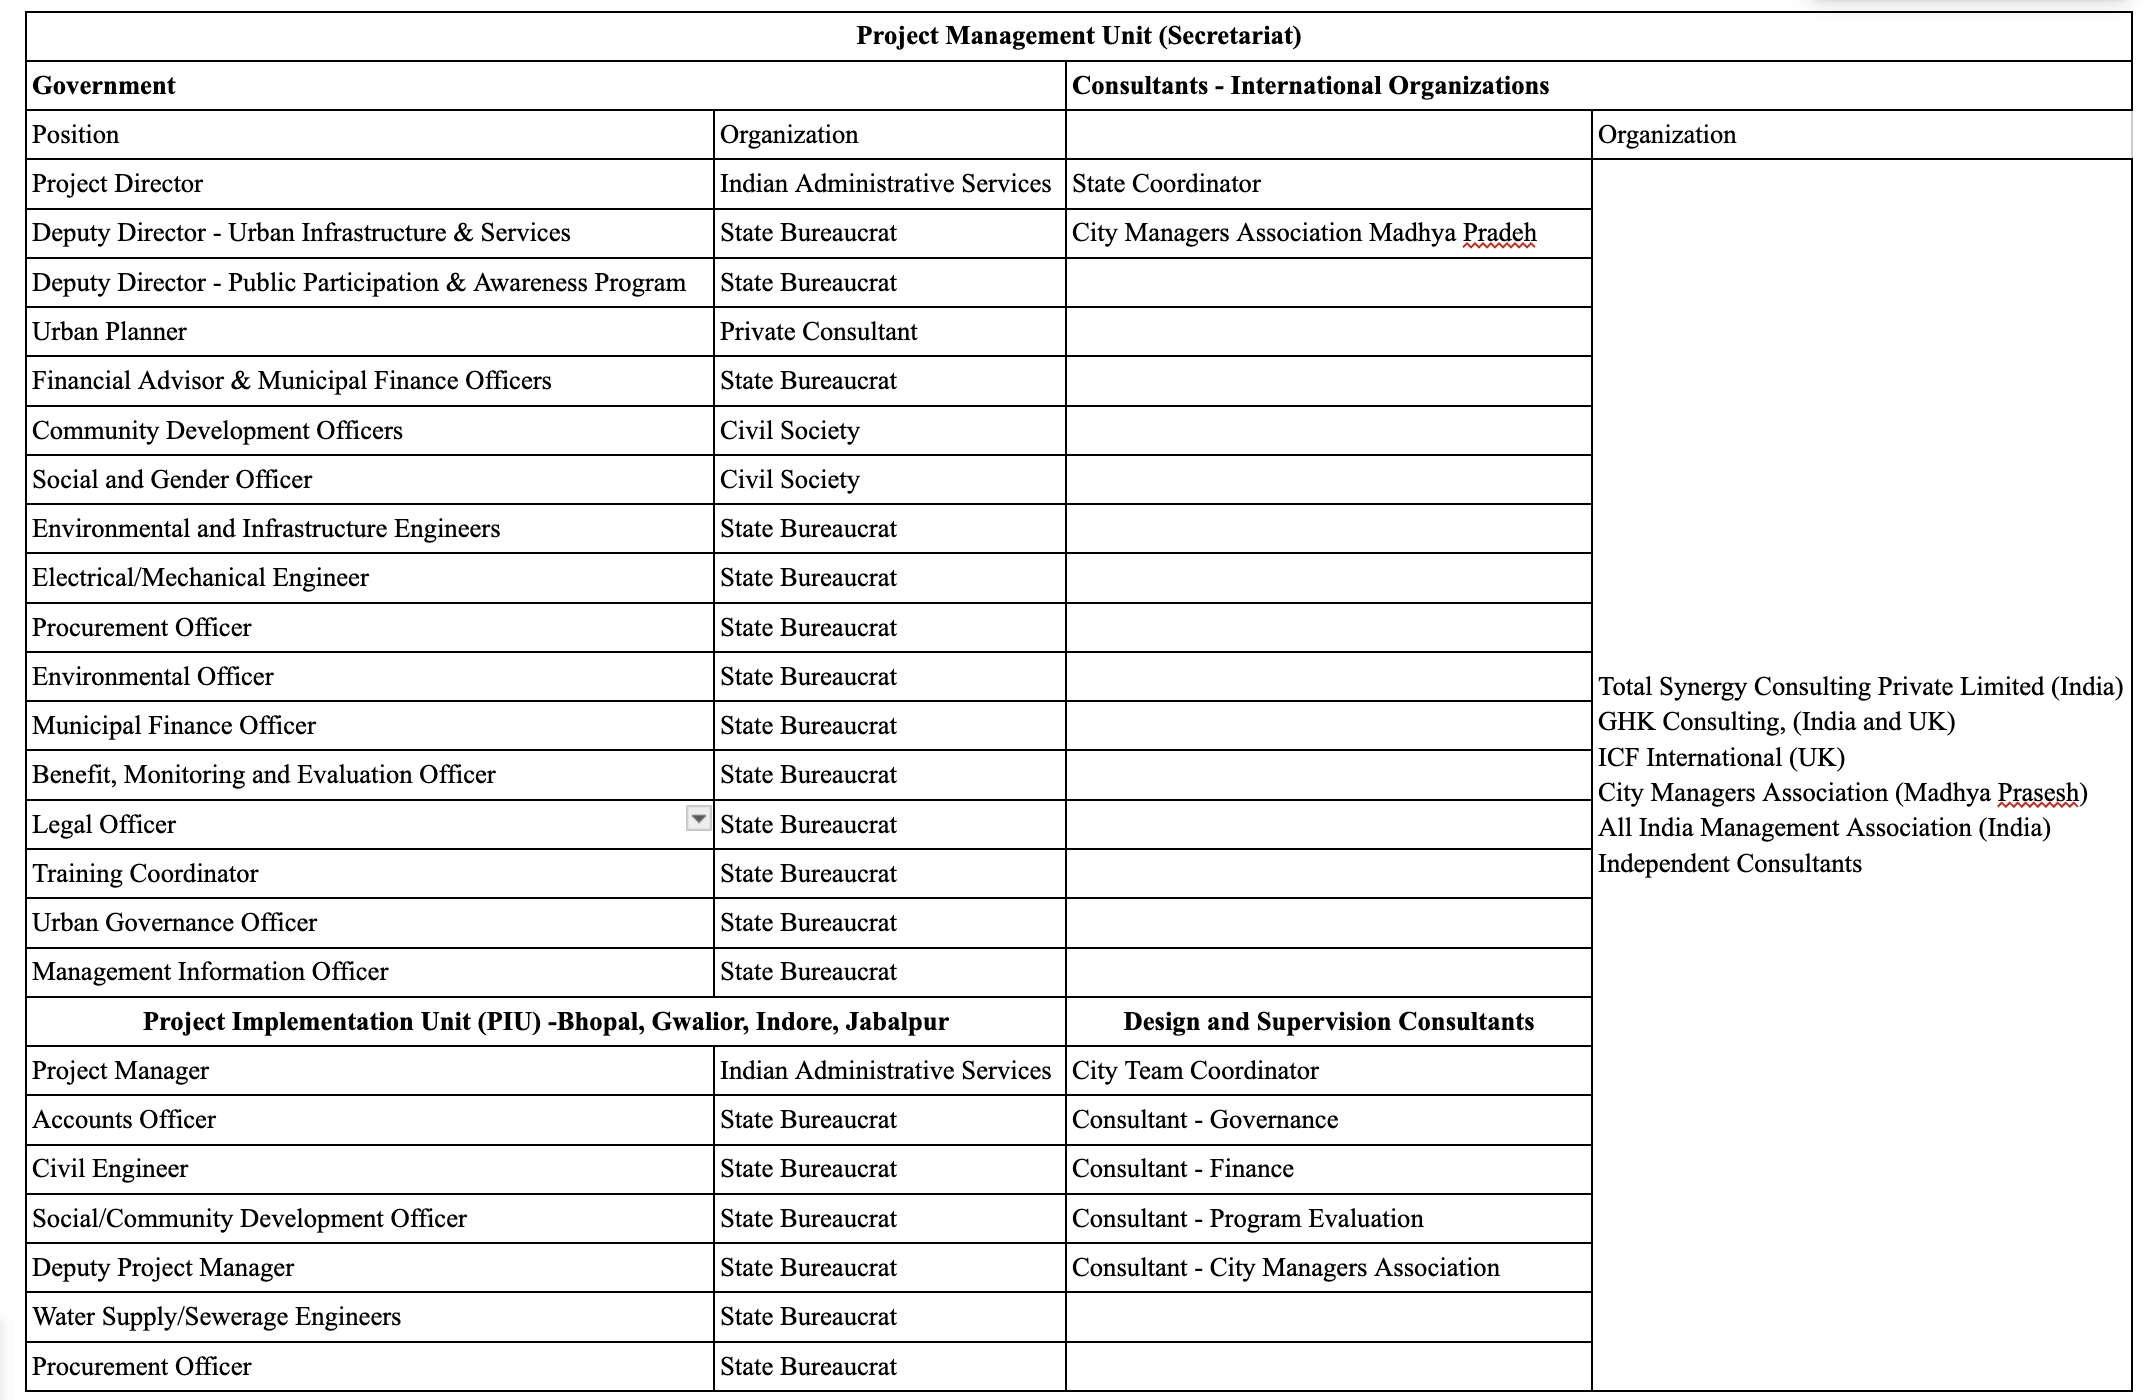
\includegraphics[width=1\textwidth]{images/ORGANOGRAM.png} % Adjust the width as needed
    \caption{Organogram under the Project Management Unit and Project Implementation Unit - 2005-2016. Source Primary Field work and \url{https://web.archive.org/web/20180829001059/http://projectuday.gov.in/Organisation.htm}}
   
\end{figure}

\subsection{Results from Citizen Survey}

The quantitative analysis of water access in Bhopal and Lucknow, drawn from the city-representative survey (n=3,754), provides compelling evidence of both city-level disparities and the critical role of political networks. The logistic regression results show that residents of Lucknow are at a distinct disadvantage compared to those in Bhopal when it comes to accessing water services. Specifically, the regression coefficient for the city dummy variable is -0.830, which translates to significantly lower odds of receiving water. When converted into odds ratios, this finding reveals that residents in Lucknow face a 56\% reduction in odds relative to Bhopal, controlling for other socio-economic and political factors (Table).  

The analysis also underscores the profound influence of political networks on water access. The regression indicates that knowing a politician personally increases the odds of receiving water, with the coefficient 0.882 translating into an odds ratio of 2.42. In other words, residents who have connections to politicians are more than twice as likely to secure water services as those without such ties. This result is further clarified by the predicted margins plot, which offers an intuitive understanding of the probabilities (Figure). For residents in Lucknow, the likelihood of receiving water remains low—around 45\%—for those who do not have any political connections. However, this probability increases sharply to approximately 88\% for individuals who know a politician personally. The nearly 43 percentage point difference highlights the systemic advantage conferred by political patronage.  

Together, these findings reveal a deeply politicized landscape of water provisioning in Lucknow, where access is shaped not just by infrastructural constraints but by one's position within political networks. 


\begin{table}[H]
\centering
\footnotesize  % This reduces the table size by approximately 1 point
\caption{Regression Results for Water in Bhopal and Lucknow}
\begin{tabular}{lD{.}{.}{-1}D{.}{.}{-1}D{.}{.}{-1}}
\toprule
\textbf{Independent Variables} & \multicolumn{1}{c}{\textbf{Full Sample}} & \multicolumn{1}{c}{\textbf{Bhopal}} & \multicolumn{1}{c}{\textbf{Lucknow}} \\
\midrule
City Dummy: Lucknow        & -0.830^{***}  &     &     \\
                           & (0.0852)      &     &     \\
Religion: Muslim           & -0.149^{*}    & 0.137       & -0.258^{**} \\
                           & (0.0858)      & (0.132)     & (0.127)     \\
Caste: OBC                 & -0.0281       & 0.148       & -0.125      \\
                           & (0.0801)      & (0.127)     & (0.111)     \\
Caste: SC                  & -0.367^{***}  & -0.315^{*}  & -0.399^{**} \\
                           & (0.118)       & (0.170)     & (0.182)     \\
Assets                     & 0.347^{***}   & -0.160      & 0.878^{***} \\
                           & (0.0775)      & (0.114)     & (0.110)     \\
Political Engagement Beyond Voting & -0.154 & 0.228       & -0.502^{***} \\
                           & (0.113)       & (0.205)     & (0.156)     \\
Effective Number of Parties & -0.197^{***} & -0.0594     & -0.268^{***} \\
                           & (0.0410)      & (0.0867)    & (0.0508)    \\
Know a Bureaucrat Personally & -0.236^{***} & -0.0831     & -0.129      \\
                           & (0.0891)      & (0.130)     & (0.132)     \\
Know a Politician Personally & -0.0234      & -1.072^{***}& 0.882^{***} \\
                           & (0.145)       & (0.202)     & (0.207)     \\
Know Both Personally        & 0.178        & -0.189      & 0.407^{**}  \\
                           & (0.140)       & (0.303)     & (0.165)     \\
Constant                    & 0.992^{***}  & 1.994^{***} & -0.158      \\
                           & (0.231)       & (0.400)     & (0.363)     \\
\midrule
Observations                & \multicolumn{1}{c}{3,754} & \multicolumn{1}{c}{1,888} & \multicolumn{1}{c}{1,866} \\
\midrule
AIC                         & \multicolumn{1}{c}{1.224} &     &     \\
BIC                         & \multicolumn{1}{c}{-11592.766} &     &     \\
Log-Lik Full Model          & \multicolumn{1}{c}{-1110.05} &     &     \\
LR(22)                      & \multicolumn{1}{c}{281.179} &     &     \\
Prob \succ R                   & \multicolumn{1}{c}{0} &     &     \\
Adj Count R2                & \multicolumn{1}{c}{0.138} &     &     \\
\bottomrule
\end{tabular}
\vspace{1em}  % Adds vertical space between the table and the footnote
\caption*{\footnotesize Robust standard errors in parentheses. \\ *** p\textless 0.01, ** p\textless 0.05, * p\textless 0.1.}
\end{table}

\begin{figure}[H] % Use [H] to force the image to appear exactly where you place it
    \centering
    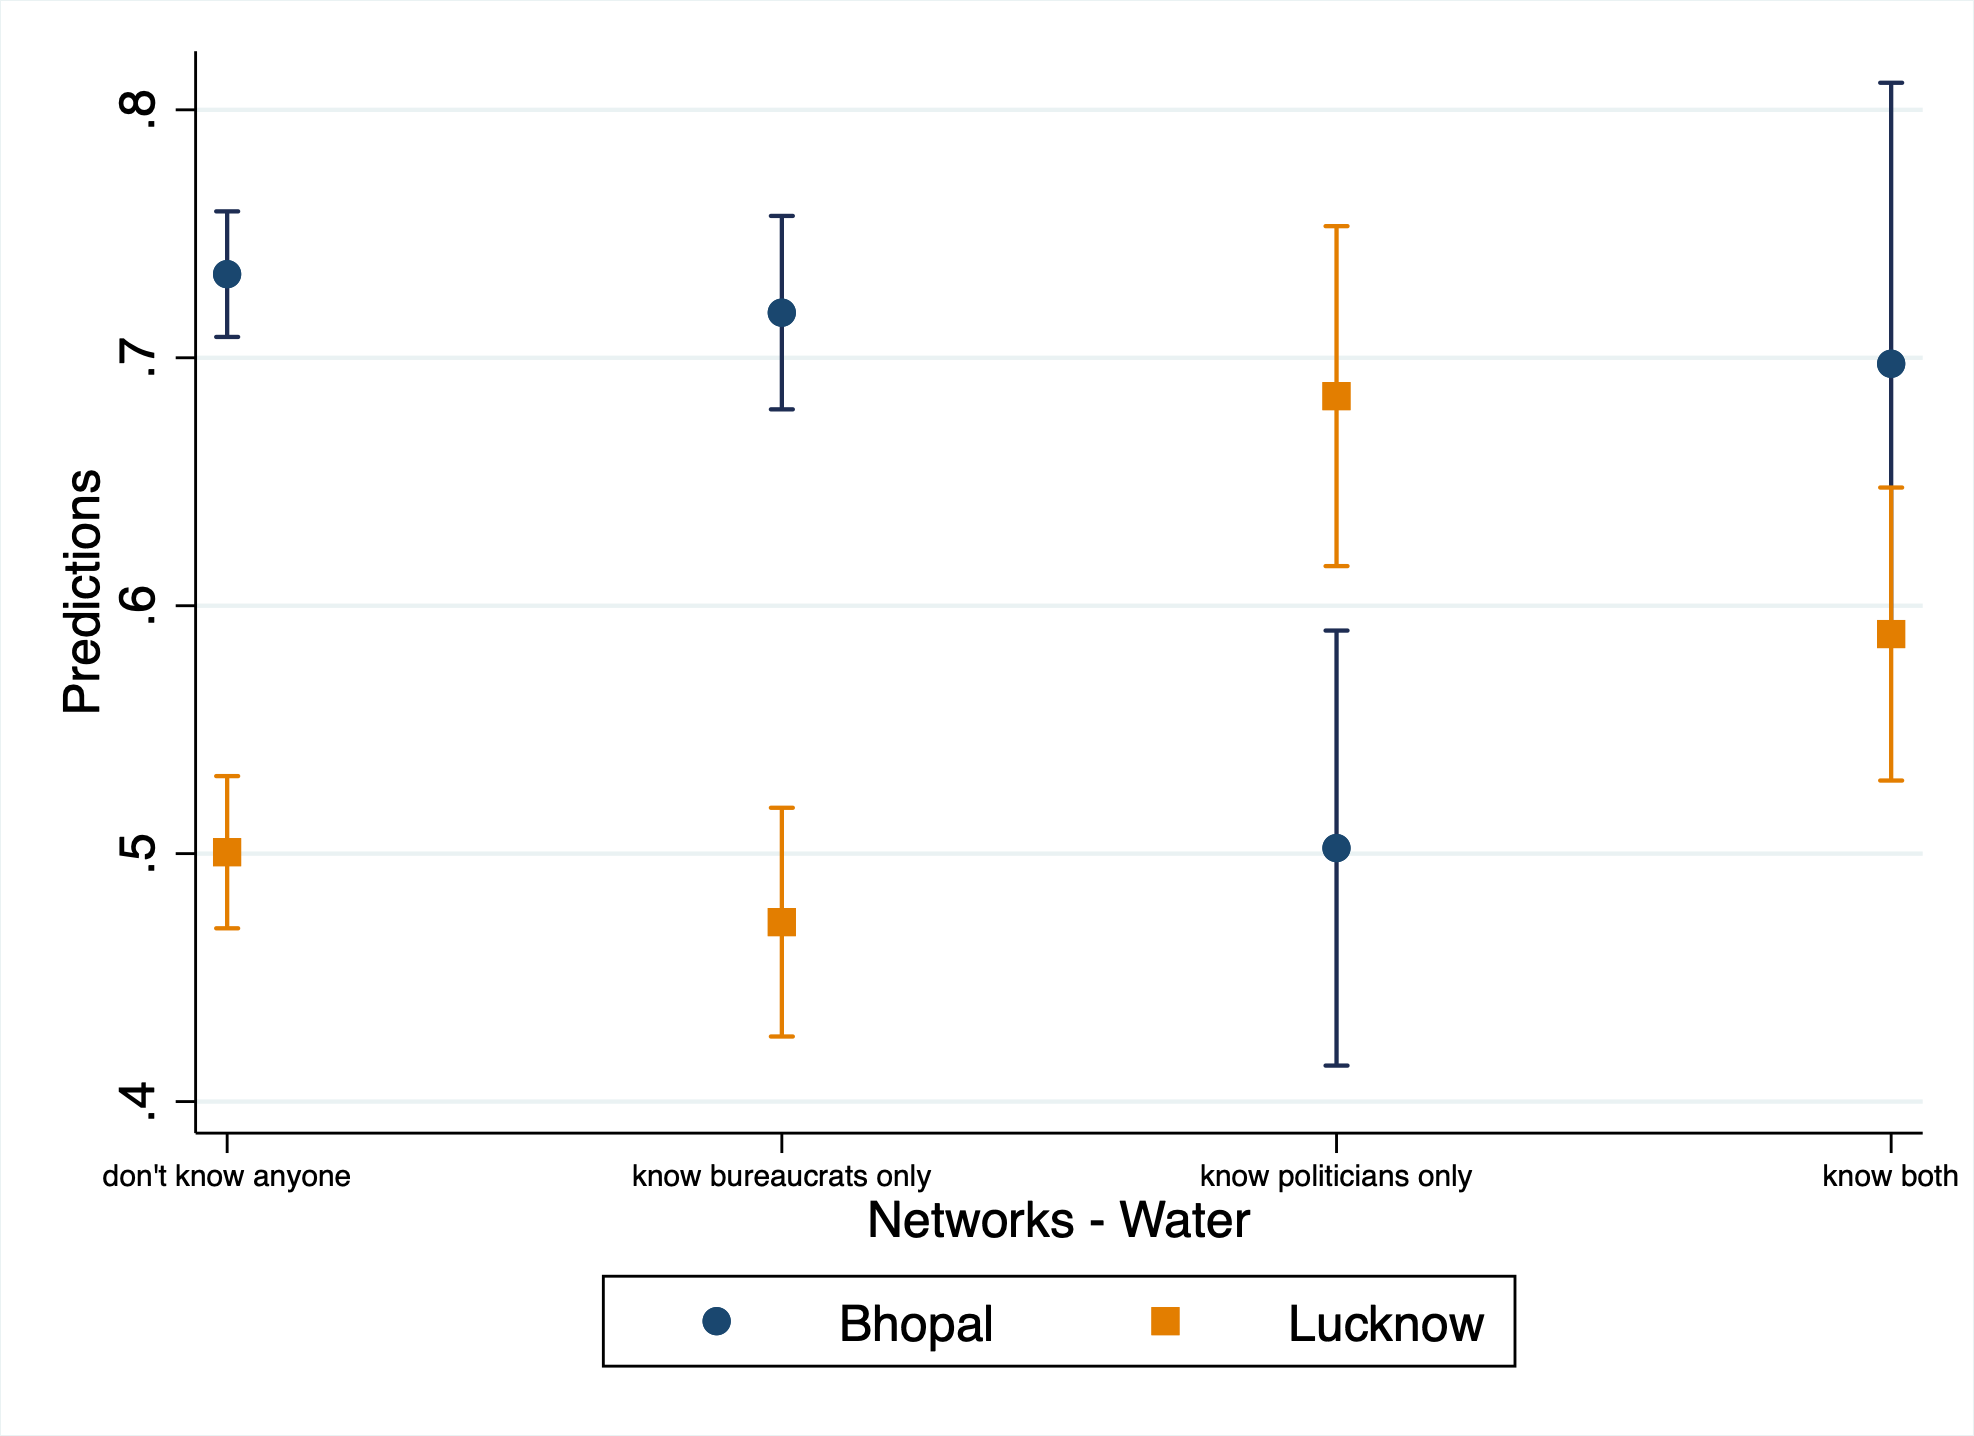
\includegraphics[width=1\textwidth]{images/Networks_water.png} % Adjust the width as needed
    \caption{This figure illustrates the predicted marginal effects of network connections
on access to water services for residents in Bhopal (blue circles) and Lucknow (orange
squares). The Y-axis represents the predicted margins (likelihood of receiving water ser-
vices), while the X-axis categorizes respondents based on their network connections. The
error bars represent 95\% confidence intervals.Source: Primary survey under the Brown - India Citizenship Project 2022}
   
\end{figure}



